\section{Umsetzung}
Hier noch generell was beschreiben. Was wird im folgenden gemacht.

\colorbox{yellow}{Hier fehlt was}

Die Abbildung~\ref{fig:uebersicht_zielarchitektur} auf Seite~\pageref{fig:uebersicht_zielarchitektur} veranschaulicht die
Zielarchitektur, wie sie in diesem Kapitel umgesetzt wird.

\begin{figure}[h]
    \centering
    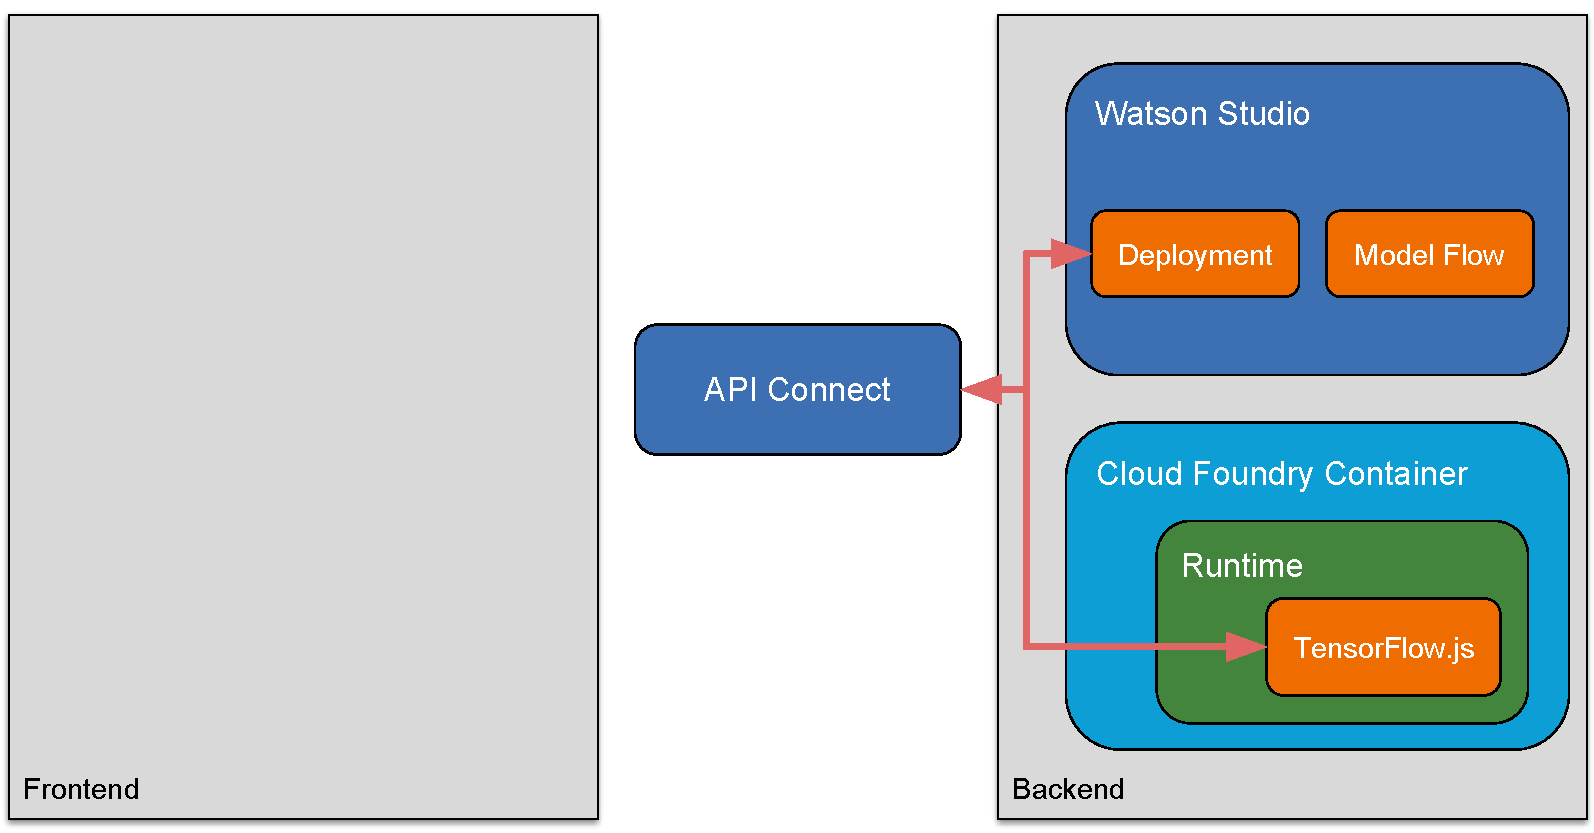
\includegraphics[scale=0.43]{images/kapitel_3/architektur_uebersicht.pdf}
    \caption{Übersicht der Zielarchitektur}
    \label{fig:uebersicht_zielarchitektur}
\end{figure}

\subsection{Cloud}
Wie in der Vorbereitung, Kapitel~\ref{sec:analyse} auf Seite~\pageref{sec:analyse}, beschrieben, wird das neuronale Netz
in der Cloud erstellt, konfiguriert und trainiert. Wie dort beschrieben, hat dies einen enormen Geschwindigkeitsvorteil
gegenüber der offline Variante. Im Anschluss daran kann das trainierte Model heruntergeladen und mit einem
TensorFlow.js-Wrapper nutzbar gemacht werden.

Die folgenden Kapitel beschreiben die dafür notwendigen Schritte und Aktionen die dürchgeführt werden müssen.

\subsubsection{Daten zusammenstellen}
\colorbox{yellow}{Hier fehlt was}

\subsubsection{Daten importieren}
Nachdem man die Trainingsdaten zusammengestellt hat, kann man diese nun in das Watson Studio importieren. Dazu existiert
in Watson Studio Dashboard einen Menüpunkt mit dem Namen \textit{Assets}.

Dieser beinhaltet alle hochgeladenen, generierten oder gesamelten Daten, Modelle, Dashboards, Notebooks oder Flows. Die
oberste Kategorie, \textit{Data Assets}, listet alle Trainingsdaten in Form von Excel-Tabellen für die Weiterverarbeitung
auf.

Über den Menüpunkt \texttt{New data asset} wird eine neue Datei hochladen. Ein klick auf diesen Menüpunkt öffnet einen
seitlichen Arbeitsbereich. Der Nutzer kann über den Menüpunkt \texttt{Browse} die Dateiauswahl des Betriebssystems
öffnen und seine Datei auswählen. Bei der Auswahl handelt es sich um die im vorangegangenen Kapitel erstellte Datei mit
Trainingsdaten.

Alternativ kann man die Datei auch in das fabrlich hervorgehobene Feld schieben. Der Upload startet damit sofort.

Nach wenigen Sekunden ist die Datei hochgeladen und wird im Bereich \textit{Data assets} angezeigt. Damit ist der
Uploadvorgang erfolgreich abgeschlossen und die Datei kann im nächsten Schritt umgewandelt werden.

\subsubsection{Daten umwandeln}
Da die erstellte Datei mit den Trainigsdaten nun in Watson Studio bereitsteht, ist die Umwandlung in eine CSV-Datei
möglich. Dieser Schritt ist zwingend notwendig, damit die Datei später als Eingabeparameter für das neuronale Netz dienen
kann. Ein anderes Format wird als Eingabe zur Zeit nicht unterstützt.

In Watson Studio liegt mit den \textit{Data flows} ein einfaches Werkzeug bereit, um Dateien in das benötigte CSV-Format
zu überführen. Dazu wird in der Kategorie Data flows über \texttt{New data flow} ein neuer Flow angelegt.

Im folgenden öffnet sich der Wizzard zum Erstellen des Flows. Der Nutzer muss im im linken Bereich die umzuwandelnde Datei
auswählen. Über die Schaltfläche \texttt{Add} wird die Auswahl dann übernommen.

Nun ist der Inhalt der Datei sichtbar. Bei der Ansicht ist darauf zu achten, dass die Werte der einzelnen Spalten als
Dezimal-Zahl interpretiert werden. Sollte diese Einstellung nicht voreingestellt sein, muss dieses Manuell abgeändert
werden.

Dazu klickt man in der entsprechenden Spalte oben auf die drei Punkte (Esintellungen) und selektiert den Eintrag
\texttt{Convert Column}. Im Untermenü muss dann der Wert \texttt{Decimal} bestätigt werden.

Da es sich nun um Dezimal-Zahlen handelt, kann man über die Schaltfläche \texttt{Run data flow} die Konvertierung starten.
Bevor die Konvertierung jedoch startet, zeigt das System eine Übersicht über die einzelnen Schritte, die dazu benötigt
werden, an.

Hier werden zum Beispiel etwaige Konvertierungen zu Dezimal-Zahlen angezeigt oder sonstige Operationen dargestellt. Der
Nutzer kann die Seite bestätigen und der Flow startet.

Nach wenigen Minuten sollte im Watson Studio im Bereich Assets, in der Kategorie Data assets, die neue Datei zur Verfügung
stehen. Dabei trägt die Datei die Dateiendung csv. Die Konvertiedung der Datei ist somit abgeschlossen und sie kann für
das neuronale Netz verwendet werden.

\subsubsection{Modeler flow}
\label{subsub:modeler_flow}
Nach erfolgreicher Konvertierung der Trainingsdaten, können diese für das neuronale Netz genutzt werden. Für die
Erstellung des neuronalen Netzes und den damit verbundenen Parameterübergaben wird der \texttt{Modeler flow} genutzt.

Über die Schaltfläche \texttt{New flow} im Bereich Assets erstellt man diesen und richtet ihn ein. Nachdem man einen Namen
und eine optionale Beschreibung für den Flow eingegeben hat, muss man die Auswahl \textit{Modeler flow} und
\textit{IBM SPSS Modeler} bestätigen. Dabei handelt es sich um den Standard-Flow von Watson Studio.

Der Nutzer bestätigt die Eingabe über die Schaltfläche \texttt{Create}. Nach kurzer Zeit ist der Flow erstellt und es
erscheint ein leerer Arbeitsbereich.

Der Menüpunkt \texttt{Palette} zeigt einen linken Arbeitsbereich an, welcher alle Module, die genutzt werden können,
gruppiert auflistet. In diesem muss man den Baustein \textit{Data asset} in der Gruppe \textit{Import} auswählen. Dieser
ermöglicht den Import der konvertierten Trainingsdaten für das neuronale Netz. Über Drag\&Drop kann der Nutzer den
Baustein in den noch leeren Arbeitsbereich platzieren.

Um den Baustein zu konfigurieren klickt der Entwickler doppelt auf den Baustein. Dies öffnet einen seitlichen
Arbeitsbereich. In diesem kann er über die Schaltfläche \texttt{Change Data Asset} die Datei auswählen, welche die
Trainingssätzen enthält. Über \texttt{Save} wird die Einstellung gespeichert und der Baustein ist fertig konfiguriert.

Im nächsten Schritt muss das neuronale Netz konfiguriert werden. Dazu existiert in der Kategorie \textit{Modeling} das
Modul \textit{Neural Net}. Dies stellt für die Anwendung die beste Alternative dar. Genau wie das Import-Modul kann dieses
mit der Maus auf ein freies Feld des Arbeitsbereiches platziert werden. Somit ist das Modul teil des Prozesses.

Damit das neuronale Netz die importierten Daten nutzen kann, wird eine Verbindung zwischen dem Import-Modul und dem
Neural-Net-Modul aufgebaut. Über einen klick auf den Ausgang des Import-Moduls kann eine Verbindungslinie gestartet werden.

Mit einem klick auf den Eingang des Neural-Net-Modul kann man die Verbindung aufbauen. Die Verbindung wird nun über eine
durchgezogene Linie zwischen den beiden Modulen visualisiert.

Bei einer Verbindung werden die Ausgaben des jeweiligen Modules weiter an die mit einer Linie verbundenen Module
gegeben. Diese Folgemodule können die Werte dann als Eingabevariablen nutzen.

Damit das Neural-Net-Modul konfiguriert werden kann, muss der Nutzer doppelt auf dieses klicken. Damit man die
\textit{Targets} und die \textit{Inputs} selbst definieren kann, muss der Hacken bei \enquote{Use custom field roles}
gesetzt werden.

Die Tabelle~\ref{tab:targets_inputs} auf Seite~\pageref{tab:targets_inputs} zeigt die auszuwählenden Tabellenspalten für
die jewielige Kategorie. Dabei beschreiben die Targets die Variablen, welche durch den Watson Service Vorhergesagt werden
sollen. Die Inputs definieren die Größen, durch welche eine Vorhersage überhaupt möglich ist.

Dem resultierenden, trainierten Model werden zu einem späteren Zeitpunkt die Inputs übergeben und die Targets kommen als
vorhergesagte Rückgabeparameter zurück.

\begin{table}[h]
    \centering
    \begin{tabular}{|c|c|}
        \hline
        \textbf{Targets} & \textbf{Inputs}\\
        \hline
        \hline
        Leistung & Einlaufbandlänge\\
        \hline
        Druckluft & Wägebandlänge\\
        \hline
        Impuls & Auslaufbandlänge\\
        \hline
        Totzeit & Einlaufbandbreite\\
        \hline
        Position & Wägebandbreite\\
        \hline
        & Auslaufbandbreite\\
        \hline
        & Einlaufbandrolle\\
        \hline
        & Wägebandrolle\\
        \hline
        & Auslaufbandrolle\\
        \hline
        & Produktbreite\\
        \hline
        & Produktlänge\\
        \hline
        & Produkthöhe\\
        \hline
        & Packungsgewicht\\
        \hline
    \end{tabular}
    \caption{Variablen für die Targets und Inputs}
    \label{tab:targets_inputs}
\end{table}

Mit dieser Konfiguration werden 13 Parameter als Eingabevariablen genutzt und fünf Parameter durch das neuronale Netz
vorhergesagt. Vier der Vorhergesagten Parameter (Druckluft, Impuls, Totzeit, Position) beziehen sich auf den
\textit{Pusher} und der Parameter \textit{Leistung} gibt die tatsächliche Bandgeschwindigkeit an, mit der das Band in der
Maschine laufen soll.

Alle anderen Einstellungen des neuronalen Netzes werden im ersten Schritt auf den Standardeinstellungen belassen. Zu einem
späteren Zeitpunkt, wenn sich Testdaten ändern oder Parameter angepasst werden müssen, kann man mit den weiteren
Einstellungen das neuronale Netz anpassen.

Der Flow für das neuronale Netz ist somit fertiggestellt. Mit einem klick auf \texttt{Run} startet das Training des
neuronalen Netzes.

Nach dem erfolgreichem training des neuronalen Netzes erscheint das trainierte Model unterhalb des neuronalen Netzes im
aktuellen Arbeitsbereich. Eine gestrichelte Linie zwischen dem neuronalen Netz und dem trainierten Model zeigt die
Abhängigkeit der beiden Module an.

Für die Weiterverarbeitung und ein späteres Deployment des trainierten Models muss man dieses mit einem Export-Modul
verbinden. Der Export erfolgt über das Modul \textit{Table}.

Das Table-Modul befindet sich in der Kategorie \textit{Outputs} und wird, genau wie alle andere Module, frei auf dem
Arbeitsbereich platziert. Eine Verbindung zwischen dem trainierten Model und der Table ermöglicht den Datenaustausch.
Für die Table ist keine weitere Konfiguration notwendig.

Ein rechtsklick auf das Table-Modul öffnet das Kontextmenü des Moduls. Darüber lässt sich der Punkt
\enquote{Save branch as a model} anklicken. Dieser ermöglicht es, das trainierte Model zu exportieren.

In dem sich öffnenden Fenster muss man den Namen und eine optinale Beschreibung für das neue Model definieren. Mit einem
klick auf den Button \texttt{Save} wird das Model gespeichert und es erscheint im Watson Studio Dashboard.

In der Abbildung~\ref{fig:umsetzung_model_flow} auf Seite~\pageref{fig:umsetzung_model_flow} ist der vollständige Aufbau
des Model flows visualisiert.

\begin{figure}[h]
    \centering
    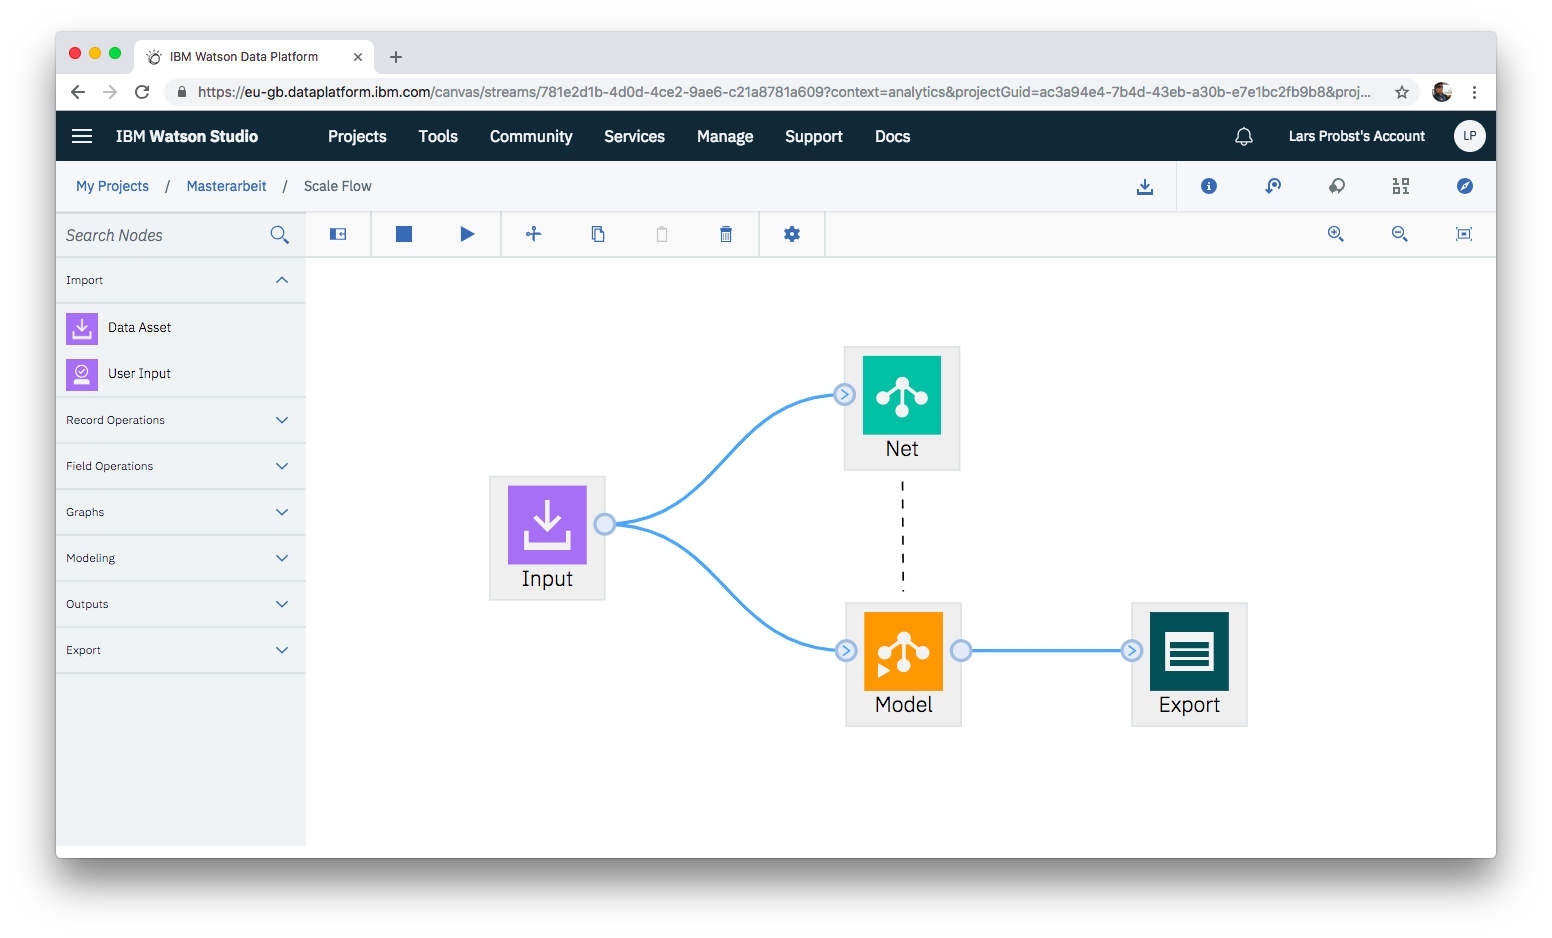
\includegraphics[width=\textwidth]{images/kapitel_3/umsetzung_model_flow.png}
    \caption{Vollständiger Model flow}
    \label{fig:umsetzung_model_flow}
\end{figure}

\subsubsection{Informationen zum Model}
Über einen weiteren rechtsklick auf das trainierte Model kann man über den Menüpunkt \texttt{View Model} auf eine
detaillierte Übersicht des Models gelangen. Hier finden sich zahlreiche Informationen, die unter anderem Aufschluss
über die Genauigkeit des Models geben.

Die erste Information, welche man als Benutzer über das Model zu sehen bekommt, ist in
Abbildung~\ref{fig:umsetzung_model_evaluation} auf Seite~\pageref{fig:umsetzung_model_evaluation} zu sehen \textendash{}
die \texttt{Evaluation}.

\begin{figure}[h]
    \centering
    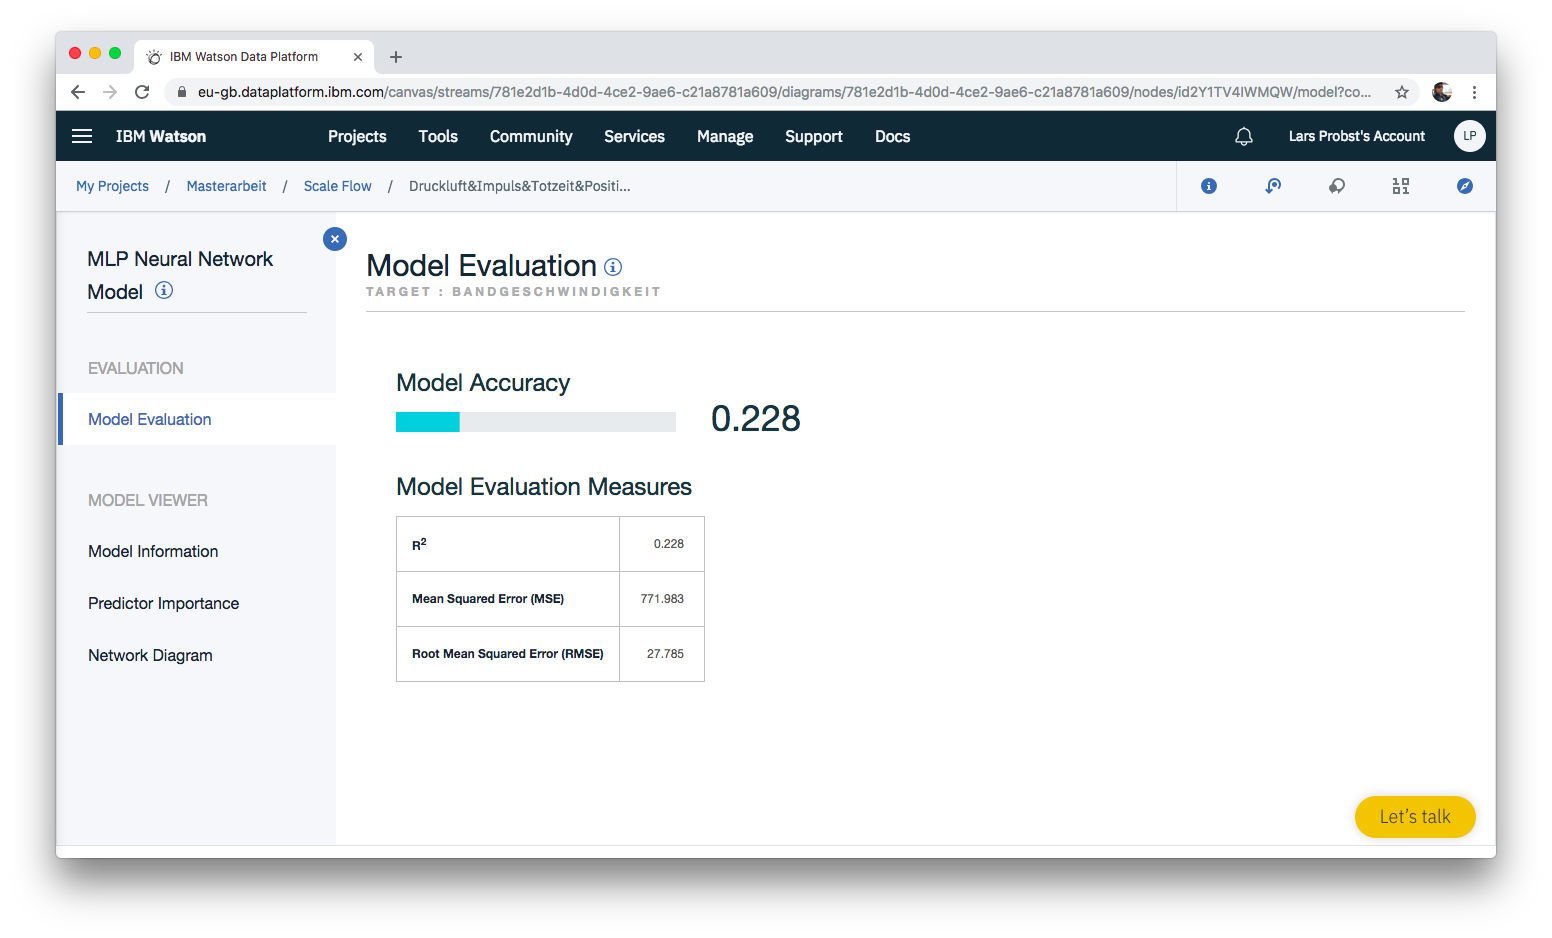
\includegraphics[width=\textwidth]{images/kapitel_3/model_evaluation.png}
    \caption{Kompletter Model flow}
    \label{fig:umsetzung_model_evaluation}
\end{figure}

Die große Zahl gibt die Genauigkeit des Models (englisch Model Accuracy) an. Mit 100 Multipliziert erhält man die
prozentuale Angabe der Genauigkeit. Wenn man mit dem Mauszeiger über die Zahl fährt, erhält man eine genauere Angabe.

Die Genauigkeit berechnet sich durch ein Testdatenset, welches dem Trainingsdatenset entnommen wird. Dabei kann beim
trainieren des Models angegeben werden, um wie viele es sich handeln soll.

Nachdem das Model fertig trainiert ist, wird es mit den zur Verfügung stehenden Testdaten gefüttert. Im Anschluss werden
die vorhergesagten Werte mit denen im Testdatenset verglichen. Je größer die Abweichung ist, desto geringer ist die
Genauigkeit.

Im weiteren finden sich Bewertungskreterien für das trainierte Model (englisch Model Evaluation Measures). Diese geben
Aufschluss darüber, wie gut das Model ist. In der ersten Zeile wird zum Beispiel $\mathbf{R^2}$ ausgegeben.  Dabei
handelt es sich um den Determinationskoeffizient. Dieser ist eine wichtige Kennzahl zur formalen Beurteilung der
Regression. Weitere Informationen sind auf der Wikipedia-Seite\footnote{https://de.wikipedia.org/wiki/Bestimmtheitsmaß}
ersichtlich.

Der nächste Wert entspricht der Mittleren quadratische Abweichung (englisch Mean Squared Error). Dies ist der Durchschnitt
der quadrierten Fehler. Als Fehler ist die Differenz der vorhergesagten Werte und der tatsächlichen Werte definiert.

Der letzte Wert gibt die Mittleres Abweichungsquadrat (englisch Root Mean Squared Error) an. Dieser Wert ist ein Maß
für die Unterschiede zwischen Werten, die von einem Modell vorhergesagt werden, und den tatsächlich beobachteten Werten.

In der nächsten Kategorie, Model Viewer, sind Informationen zu den einzelnen Werten des neuronalen Netzes angegeben.
Unter dem ersten Menüpunkt, können alle Informationen gefunden werden.

Mit einem Klick auf den Menüpunkt, gelangt man in eine Ansicht wie in Abbildung~\ref{fig:umsetzung_model_information}
auf Seite~\pageref{fig:umsetzung_model_information} zu sehen.

\begin{figure}[h]
    \centering
    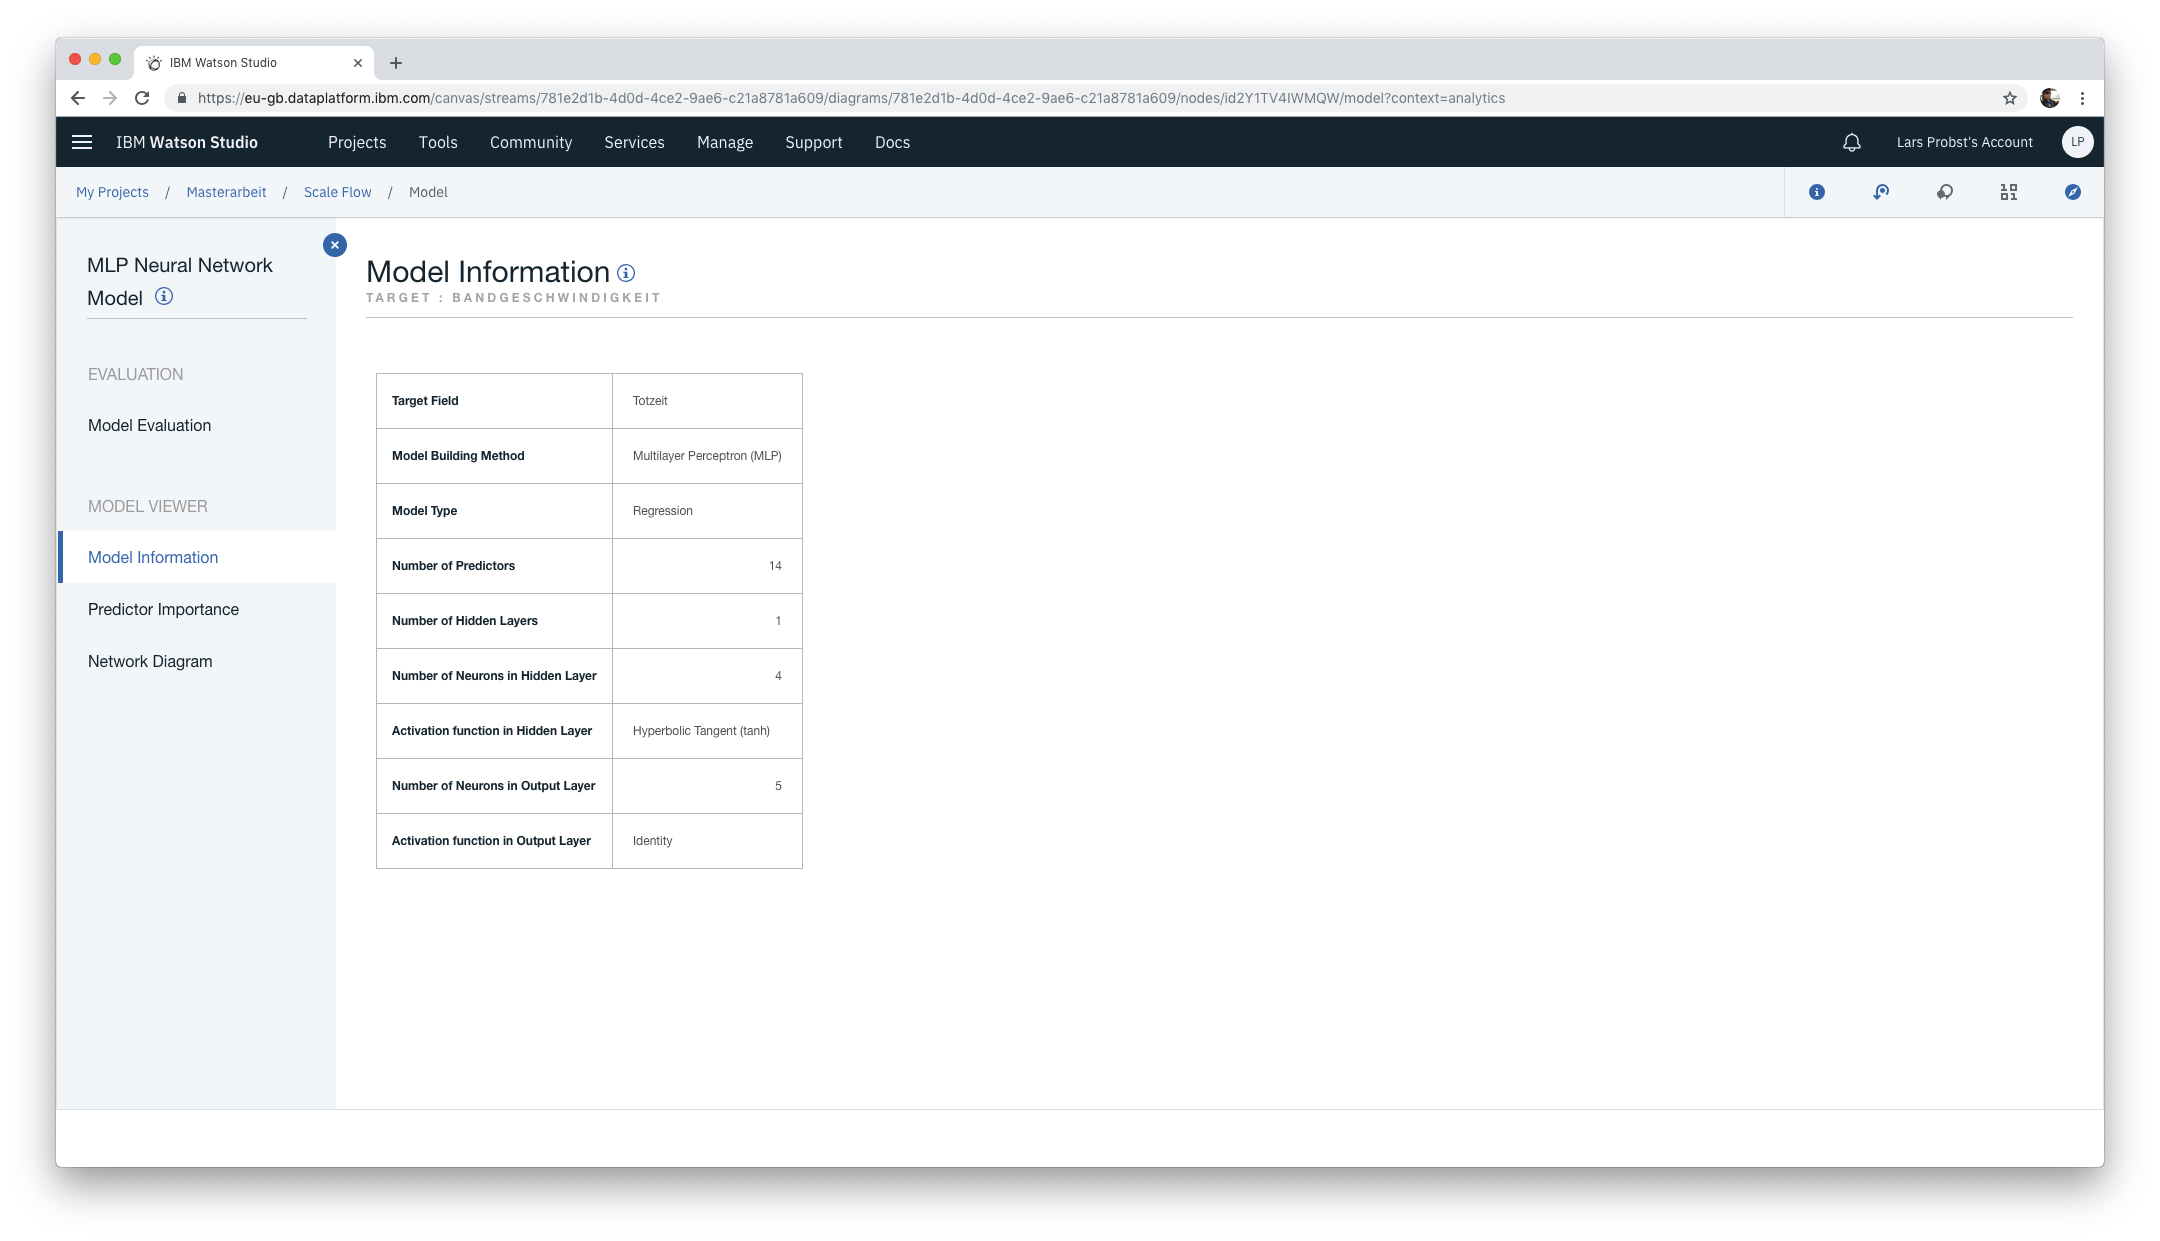
\includegraphics[width=\textwidth]{images/kapitel_3/model_information.png}
    \caption{Kompletter Model flow}
    \label{fig:umsetzung_model_information}
\end{figure}

Hier findet man Informationen darüber, wie das trainierte Model aufgebaut ist oder um welche Art Model es sich handelt.
Auch die Hiden Layers, die im neuronalen Netz eingerichtet sind, werden hier angegegeben.

Weiter ist hier angegeben, mit wie vielen Inputparameter (englisch Number of Predictors) das Netz trainiert ist und wie
viele Ausgabewerte (englisch Number of Neurons in Output Layer) das Netz vorhersagen kann.

Im Menüpunkt \texttt{Predictor Importance} werden alle Input-Parameter aufgelistet. Ein Balken unterhalb jedes Parameters
gibt an, wie Wichtig dieser für das neuronale Netz ist. In Abbildung~\ref{fig:umsetzung_model_predictor} auf
Seite~\pageref{fig:umsetzung_model_predictor} ist dies beispielhaft aufgezeigt.

\begin{figure}[h]
    \centering
    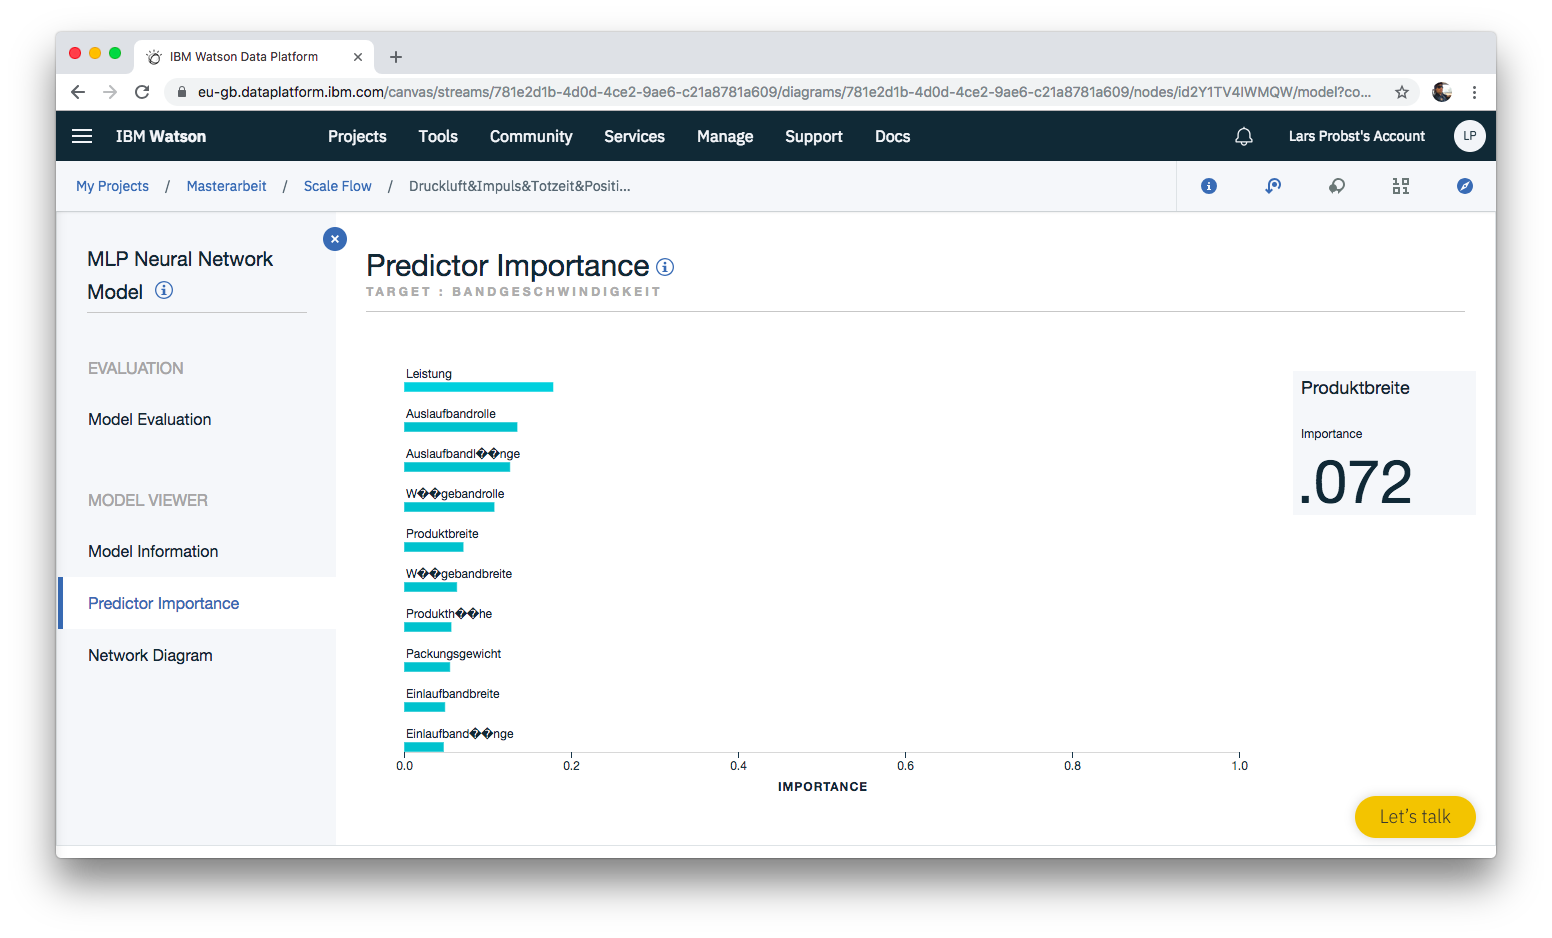
\includegraphics[width=\textwidth]{images/kapitel_3/model_predictor.png}
    \caption{Kompletter Model flow}
    \label{fig:umsetzung_model_predictor}
\end{figure}

Beim Überfahren eines Parameters wird der prozentuale Wert am rechten Rand dargestellt. Je wichtiger ein Parameter ist,
desto mehr Einfluss hat dieser auf die vorhergesagten Ausgabewerte.

Parameter mit der geringsten Gewichtung spielen für das Ergebnis keine große Rolle und könnten bei einer Optimierung des
neuronalen Netzes weggelassen werden.

Der letzte Menüpunkt, mit der Aufschrift \texttt{Network Diagram}, zeigt das neuronale Netz, wie es beim Traning aufgebaut
wurde. Dabei sind auf der linken Seite die Parameter zur Eingabe aufgelistet.

Auf der rechten Seite erscheinen die Ausgabeparameter. Dazwischen werden die \textit{Hidden Layers} dargestellt und wie
diese mit der Eingangs- und Ausgangsseite verbunden sind.

Die Abbildung~\ref{fig:umsetzung_model_network_diagram} auf~\pageref{fig:umsetzung_model_network_diagram} visualisiert
das vorangegangene, trainierte Model.

\begin{figure}[h]
    \centering
    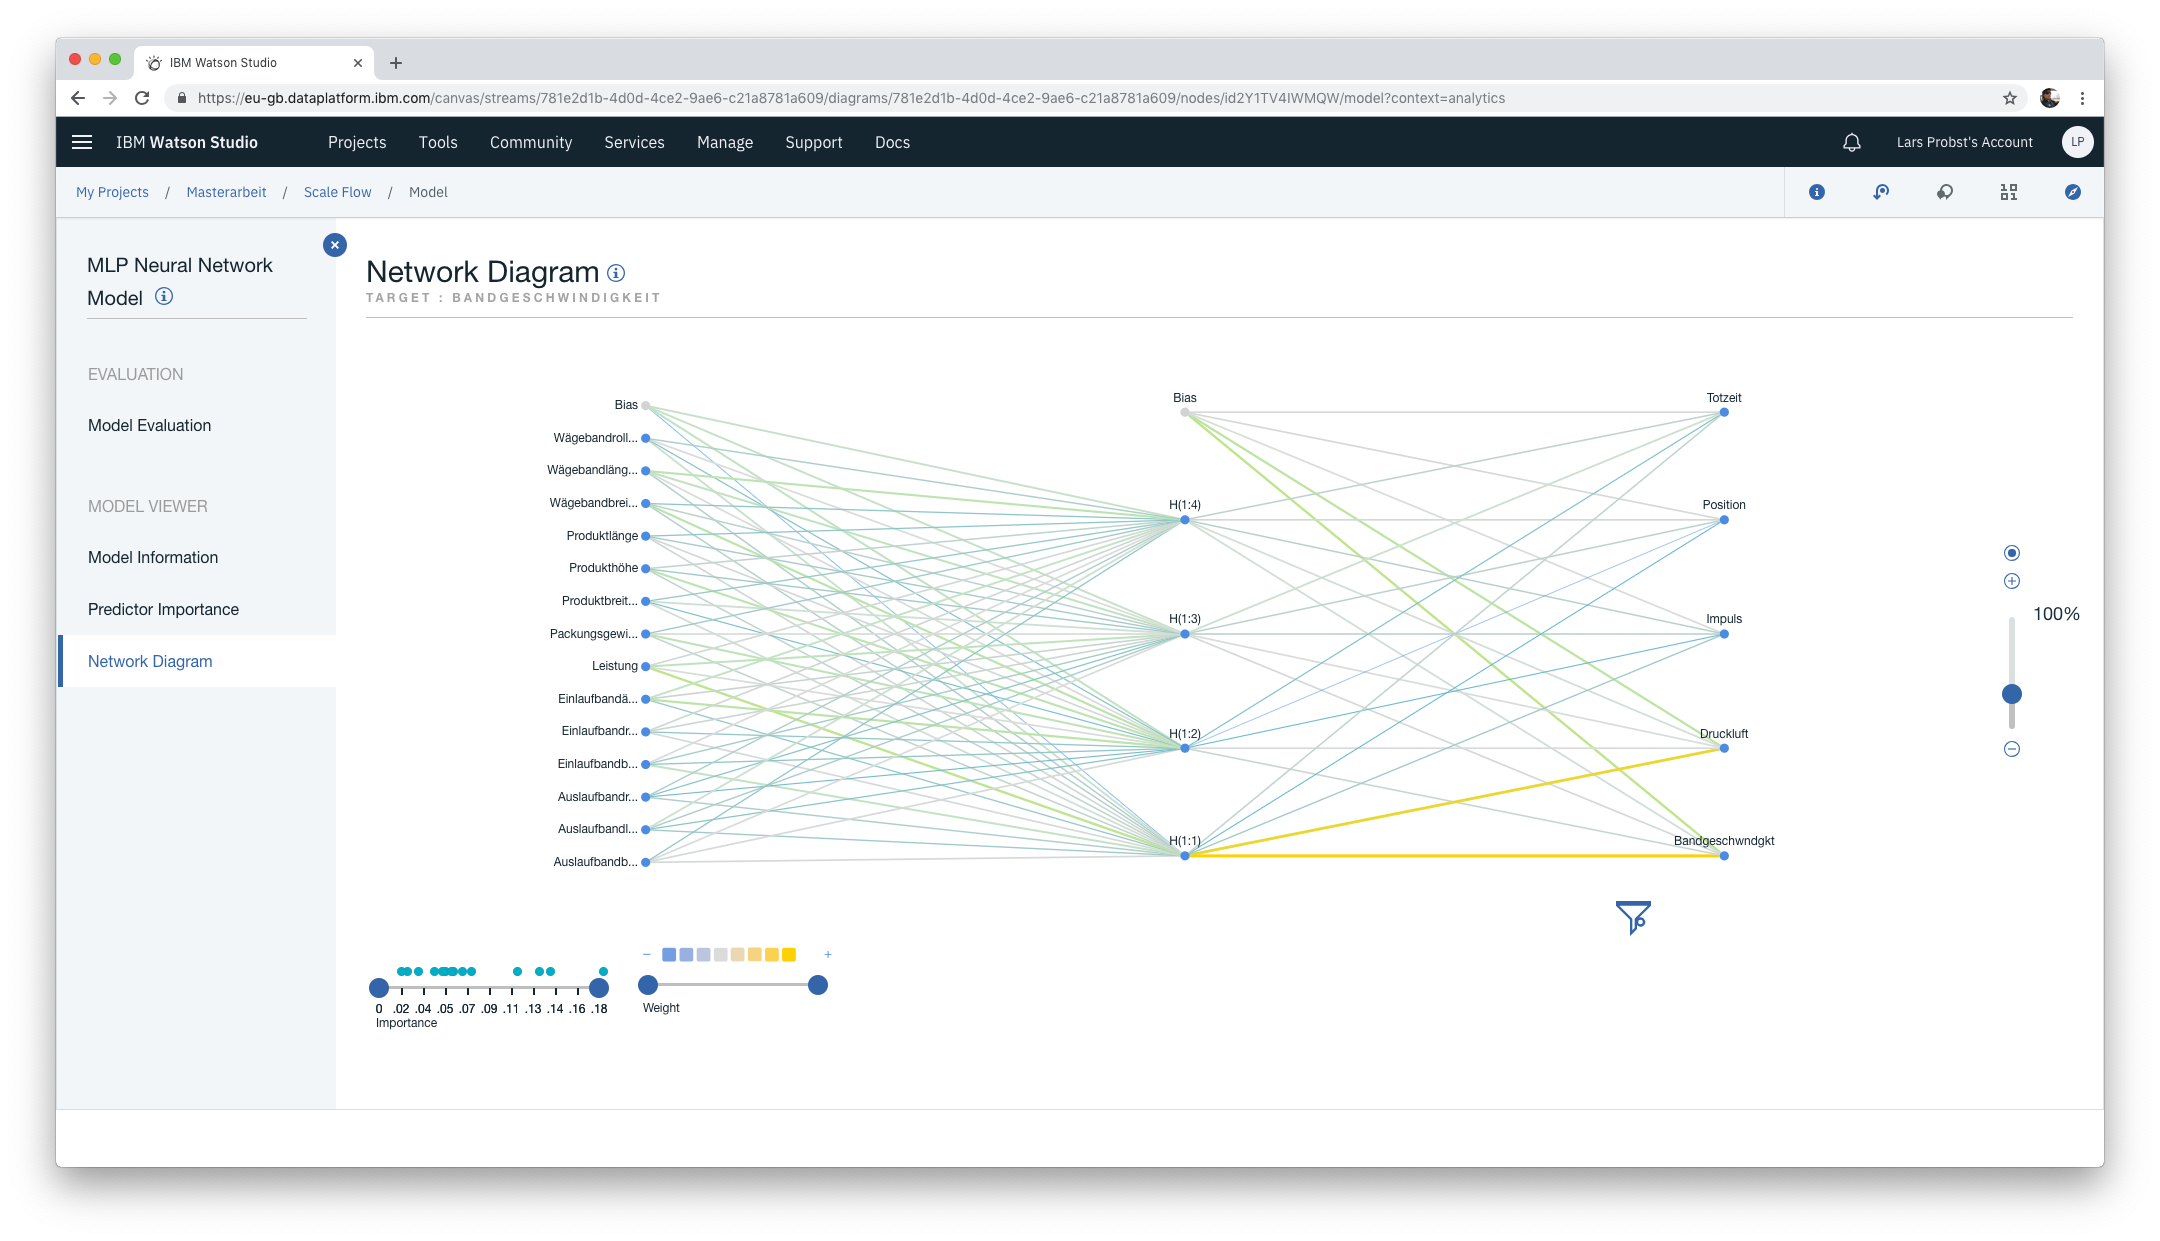
\includegraphics[width=\textwidth]{images/kapitel_3/model_network_diagram.png}
    \caption{Kompletter Model flow}
    \label{fig:umsetzung_model_network_diagram}
\end{figure}

Die Ansicht kann über einen Slider am rechten Bildschirmrand die Ansicht vergrößern oder verkleinern. Über die Legende
am unteren Rand, kann man die einzelnen Verbindungen filtern. So ist es zum Beispiel möglich, dass man sich alle
Verbindungen mit hoher Priorität anzeigen lässt. So hat der Entwickler eine Vorstellung, wie die wichtigsten
Eingabeparameter für die entsprechende Ausgabe sorgen.

Auch kann man sich so anschauen, wie einzelne Werte auf der Eingabeseite einen direkten Einfluss auf einen Ausgabewert
haben. Im Beispiel der Abbildung hat der Parameter \textit{Leistung} zum Beispiel einen direkten und sehr großen
Einfluss auf den Ausgabewert \textit{Bandgeschwindigkeit}. Was bei weiterer Betrachtung Sinn ergibt.

Wenn mehr Produkte über die Waage laufen sollen (es soll die Leistung erhöht werden), muss das Band mit höherer
Geschwindigkeit (Bandgeschwindigkeit) drehen. Desweiteren hat die Leistung einen niedrigeren Einfluss auf den Parameter
\textit{Druckluft}. Diese gibt indirekt die Geschwindigkeit an, mit welcher der Pusher ausschlagen soll um ein Produkt
vom Band zu hauen.

Was bei näherer Betrachtung auch Sinn ergibt, da eine höhere Bandgeschwindigkeit auch ein schnelleren Pusher voraussetzt,
um das Produkt auch vom Band hauen zu können.

\subsubsection{Deployment erstellen}
Das in einem vorangegangenen Kapitel erstellte und trainierte Model kann im weiteren durch ein Deployment über eine
REST-Schnittstelle verfügbar gemacht werden. Dazu ist es erforderlich, das Model in einen \texttt{Web service} zu
installieren. Die spätere Wartung und Verwaltung wird dabei von Bluemix übernommen.

Für die Erstellung des Web Services muss man im Watson Dashboard das erstellte Model auswählen. Das folgende Fenster
zeigt mehrere Informationen zu diesem an. Unter anderem ist sichtbar, welche Eingabe- und Ausgabeparameter für das Model
wichtig sind.

Der Reiter \texttt{Evaluation} zeigt vorangegangene Auswertungen des Models an. Über den Menüpunkt \texttt{Lineage}
werden Verknüpfungen und Abstammungen des Models angezeigt.

Für das Deployment ist der Reiter \texttt{Deployments} wichtig. Dieser verwaltet alle Deployments des Modules. Das Löschen
von älteren Deployments oder das Erstellen von neuen ist hier möglich. Die Schaltfläche \texttt{Add Deployment} öffnet
eine Konfigurationsseite zum Erstellen eines neuen Deployments.

Als Type für das Deployment muss man \textit{Web Service} auswählen. Der Name des Deployments ist das einzige Pflichtfeld
und muss befüllt sein. Anschließend wird das Deployment über \texttt{Save} gespeichert und gestartet. Dieser Vorgang kann
wenige Minuten dauern.

Nachdem das Deployment fertiggestellt ist, wird in der Spalte \textit{Status} der aktuelle Wert \texttt{DEPLOY\_SUCCESS}
angezeigt. Die Informationsseite des Deployments kann man über einen klick auf den Namen öffnen.

Das Deployment ist somit erfolgreich erstellt und kann im Weiteren getestet und genutzt werden.

\subsubsection{Deployment testen}
Ein online Test des eingerichteten Deployments ist über das Watson Studio Dashboard möglich. Dies hat den Vorteil, dass
man das Deployment direkt testen und bei Fehlveralten neu trainiert kann.

Auf der Deploymentseite des gespeicherten Models genügt ein klick auf den Namen um die Deploymentinformationen anzuzeigen.
Hier steht neben diversen Informationen auch der Menüpunkt \texttt{Test} zur Verfügung. In diesem öffnet sich eine
zweispaltige Ansicht.

In der linken Spalte befinden sich die Eingabefelder für das trainierte Model (die Inputs). Nachdem man alle Felder mit
Testwerten gefüllt hat, kann man über die Schaltfläche \texttt{Predict} eine Vorhersage starten.

Nach wenigen Sekunden erscheint auf der rechten Seite ein langes JSON-Object, welches den Rückgabewert des Web Services
enthält. Das erste Array, \textit{fields}, listet alle an den Web-Service gesendeten Felder auf (die Inputs).

Das zweite Array, \textit{values}, die an den Web-Service gesendeten wie auch die Vorhergesgaten Werte (die Inputs und
die Targets). Die letzten fünf Werte des Arrays entsprechen den Vorhersagen des trainierten Models (die Targets).

Sollte das Array \textit{values} kleiner sein als das Array \textit{fields}, war das trainieren des Models nicht
erfolgreich.

Unter dem Menüpunkt \texttt{Implementation} werden wichtige Informationen und erforderliche Schritte aufgezeigt, damit
man die Schnittstelle in das eigene Programm integriert kann. Dabei wird auf verschiedene Programmiersprachen eingegangen.

In Abbildung~\ref{fig:umsetzung_deployment_test} auf Seite~\pageref{fig:umsetzung_deployment_test} ist ein Beispiel für
den online Aufruf des trainierten Models sichtbar.

\begin{figure}[h]
    \centering
    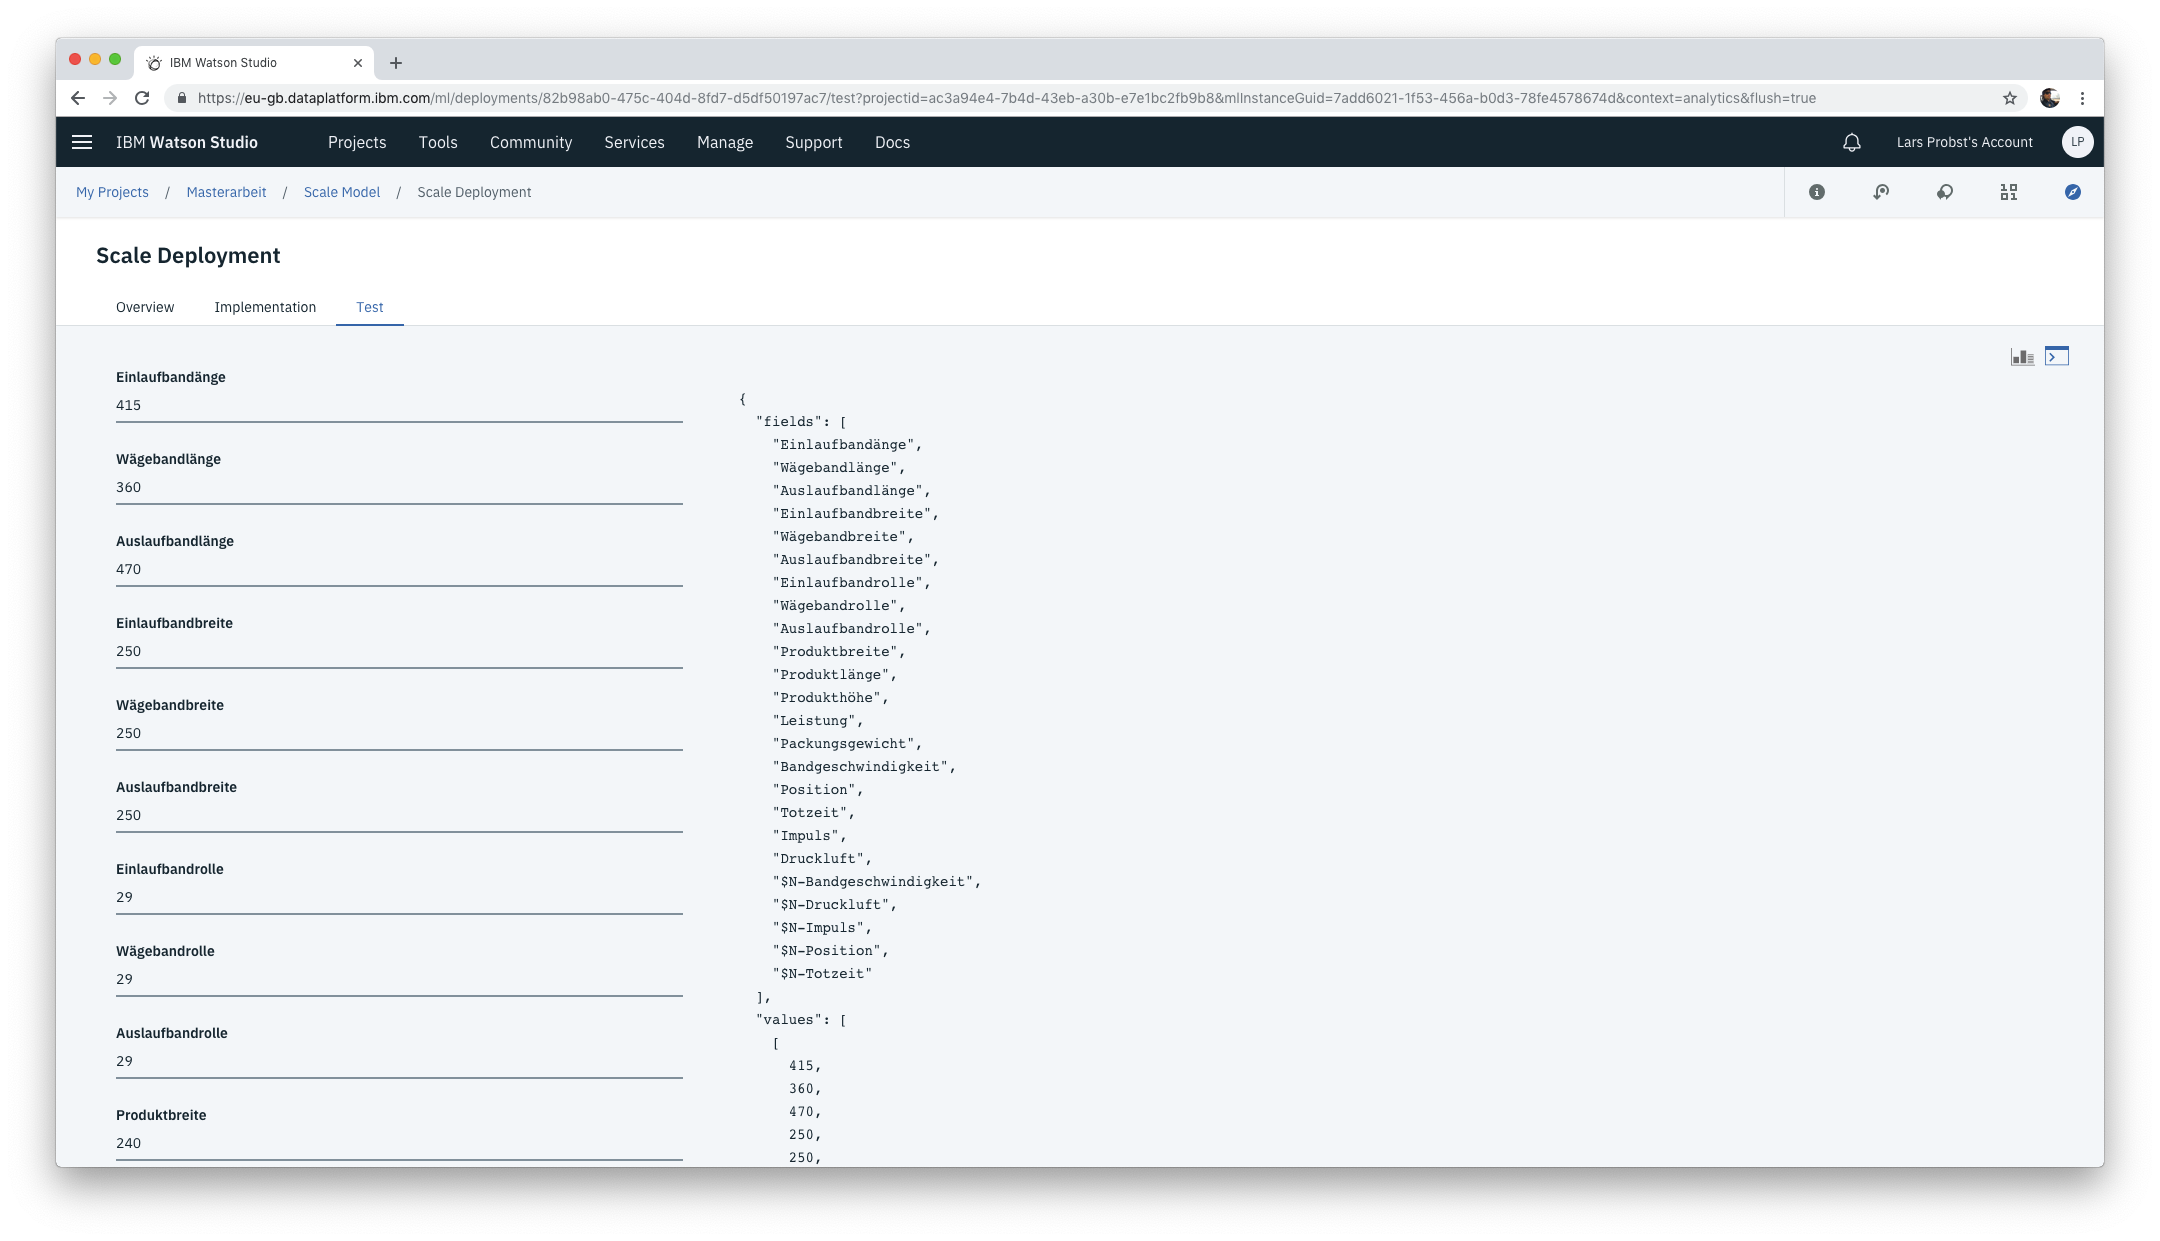
\includegraphics[width=\textwidth]{images/kapitel_3/deployment_test.png}
    \caption{Online Test des trainierten Models}
    \label{fig:umsetzung_deployment_test}
\end{figure}

\subsubsection{Aufruf mit Postman}
\label{subsec:Aufruf mit Postman}
Im Weiteren soll das erstellte Model, welches im vorherigen Kapitel als Deployment in einen Web-Service zur Verfügung
gestellt wurde mit Postman\footnote{https://www.getpostman.com} getestet werden.

So ist sichergestellt, dass man das Model auch von extern, nicht nur über das Watson Studio Dashboard, aufrufen kann.
Dies ist für die spätere Entwicklung des Frontends und die Einrichtung des API Connect Services wichtig. Außerdem ist
so eine überprüfung der Übergabeparameter sowie der Rückgabewerte an die Schnittstelle möglich.

Jeder Request an den Web-Service des trainierte Models benötigt einen \textit{Authentication Token} (kurz Auth-Token).
Dieser Token stellt sicher, dass es sich um einen gültigen Aufruf handelt.

Über die REST-Schnittstelle des Watson Studios wird der Token generriert. Dabei handelt es sich um eine andere
Schnittstelle als beim Web-Service. Der Token ist immer nur für maximal vier Stunden gültig.

Um einen Auth-Token zu erstellen, muss man den Watson Studio Benutzername und das zugehörige Passwort an die Schnittstelle
übergeben. Ein Beispielaufruf ist in Listing~\ref{Abruf des Auth-Tokens} auf Seite~\pageref{Abruf des Auth-Tokens}
zu sehen. Der Token ist dabei in einem JSON-Object im Rückgabewert enthalten.

\begin{lstlisting}[language=bash, caption=Abruf des Auth-Tokens, label=Abruf des Auth-Tokens]
$ curl --basic --user USERNAME:PASSWORD https://eu-gb.ml.cloud.ibm.com/v3/identity/token
\end{lstlisting}

In Postman kann man diesen Aufruf über die Eingabe der URL und dem HTTP-Type \texttt{GET} machen. Im Reiter
\textit{Authentication} ist der Type \textit{Basic-Auth} auszuwählen.

Im rechten Bereich sollten dann die beiden Eingabefelder für Benutzername und Passwort erscheinen. Der Nutzer muss die
geforderten Daten eingeben und kann dann den Request mit der Schaltfläche \texttt{Send} starten.

Nach wenigen Sekunden erscheint im Bereich \textit{Body} der Token in einem JSON-Objekt. Ähnlich dem Aufruf mit \textit{curl}.

Um nun das eigentliche Deployment aufzurufen, muss man einen neuen Postman-Tab öffnen. Die URL für den Endpunkt ist im
Deployment des Models zu finden und heißt \texttt{Scoring End-point}.

Nachdem die URL des Postman-Requests definiert ist, kann man als HTTP-Type \texttt{POST} auswählen. Im Bereich
\texttt{Authentication} wird der Typ auf \texttt{Baerer} abgeändert und ermöglicht die Eingabe des Tokens. Dieser Token
entspricht dem Rückgabewert des vorangegangenen Postman-Requests.

Die Auswahl des HTTP-Types \textit{POST} ermöglicht die definition des Bereichs \texttt{Body} für den Request. Dabei
handelt es sich um Parameter, welche an die Schnittstelle geschickt werden.

Als Datentyp muss man \textit{raw} und als Type \textit{JSON (application/json)} auswählen. Im Anhang
\ref{sec:postmanTestparameter} auf Seite \pageref{sec:postmanTestparameter} sind Testparameter zu finden, welche als
Eingabe genutzt werden können.

Der Nutzer kann abschließend den Request über den Button \texttt{Send} an den Web Service abschicken. Nach wneigen
Sekunden zeigt Postman den erhaltenen Response des neuronalen Netzes an. Hier sollten auch die Vorhersagen enthalten sein.

In der Abbildung \ref{fig:umsetzung_deployment_postman} auf Seite \pageref{fig:umsetzung_deployment_postman} ist ein
Beispielrequest aus Postman auf das Deployment zu sehen. Im linken Bereich sieht man das gesendete JSON-Object, mit den
Eingabevariablen. Dabei hat das JSON-Objekt die beiden geforderten Items \textit{fields} und \textit{values}.

\begin{figure}[h]
    \centering
    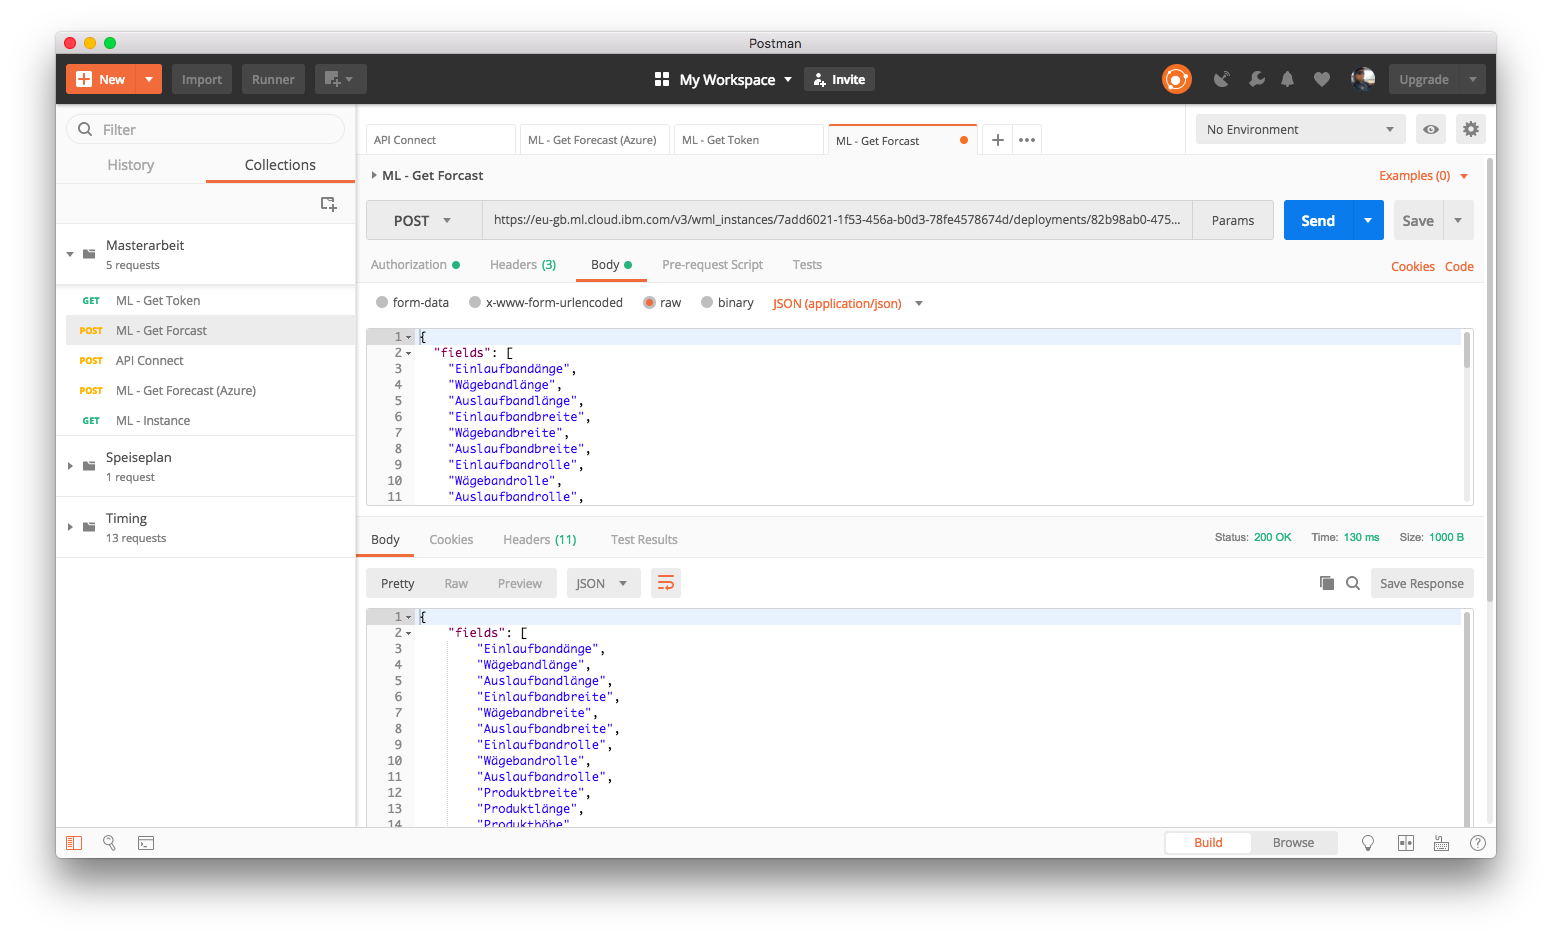
\includegraphics[width=\textwidth]{images/kapitel_3/deployment_postman.png}
    \caption{Beispielrequest von Postman}
    \label{fig:umsetzung_deployment_postman}
\end{figure}

Die Rechte Seite zeigt die Antwort des Web-Service. Dabei werden zu Anfang des JSON-Objektes die Parameter wiederholt,
die an das Interface gesendet wurden. Am Ende sind die vorhergesagten Parameter durch das trainierte Model zu sehen.

Im Eingabe-Parameter \textit{values} müssen die Output-Parameter definiert werden. Da die Werte keine Rolle spielen,
werden die Werte \textit{null} initialisiert. Damit werden sie vom System nicht weiter verwendet.

Auf der Übersichtsseite des REST-Interfaces des
Deployments\footnote{https://watson\-ml\-api.mybluemix.net/?cm\_mc\_uid=61889453441915363064337}, sind noch weitere
Endpunkte und die dafür benötigten Parameter sowie die Rückgabewerte ersichtlich.

\subsection{TensorFlow.js}
Das neuronale Netz ist nun erfolgreich in einem Deployment online zur Verfügung gestellt. Außerdem ist die Funktion
über einen Aufruf mittels Postman überprüft worden. Im Weiteren wird das trainierte Model in eine TensorFlow.js
Applikation eingebaut.

Dies hat nun mehrere Vorteile. Zum einen kann man das trainierte Model unabhängig von einer Cloud-Lösung nutzen. Die
TensorFlow-Applikation kann zum Beispiel in einen Cloud Foundry-Container geladen werden und ist somit völlig unabhängig
von der Plattform auf der die Applikation läuft. Auch kann sie modular und schnell in beliebigen Regionen instanziiert
werden.

Ein weiterer Vorteil ist die unabhängigkeit, welche damit erreichbar ist. Die Applikation kann selbst verwaltet,
instanziiert oder auch aktualisiert werden. Auch ist es möglich die TensorFlow-Applikation direkt in die Hauptapplikation
zu integrieren.

\subsubsection{Model Exportieren}
Damit das Model in die TensorFlow-Applikation eingebunden werden kann, muss es aus dem Watson Studio exportiert werden.
Dies erfolgt über den Modeler Flow.

Da das Model in Kapitel \ref{subsub:modeler_flow} auf Seite \pageref{subsub:modeler_flow} komplet trainiert wurde, steht
es im Modeler Flow als gelbes Modul bereit.

Über einen rechtsklick auf das trainierte Model und dem Menüpunkt \texttt{Download Model} kann man das Model auf den
Entwicklungsrechner herunterladen. Bei der Datei handelt es sich um eine pb-Datei. Diese Datei beinhaltet alle wichtigen
Informationen über das gebaute neuronale Netz.

Im weiteren kann mit der Entwicklung des Wrappers für das heruntergeladene neuronale Netz begonnen werden. Dafür wird
der Inhalt der Datei in einer Tensor-Flow-Applikation importiert und ausgewertet.

\subsubsection{Wrapper entwickeln}
\colorbox{yellow}{Hier fehlt was}

Die entwickelte Applikation soll im Weiteren über eine Domain aus dem Internet aufrufbar sein. Eine Installation in einen
Cloud Foundry-Container, welcher in der IBM Cloud läuft, ist dafür notwendig. Im folgenden Kapitel werden die dafür
nötigen Schritte erläutert.

\subsubsection{Toolchain einrichten}
Die fertig entwickelte Node.js-Applikation wird im nächsten Schritt in einen Cloud Foundry-Container installiert. Dies
ermöglicht den Aufruf der Applikation über eine Domain, welche automatisch von der IBM Cloud vergeben wird.

Damit der geschriebene Quellcode nicht nach jeder Änderung manuell mittels \texttt{cf push} in einen Cloud
Foundry-Container geladen werden muss, wird hierfür eine Toolchain aus der IBM Cloud genutzt.

Die Nutzung der Toolchain erfordert ein eingerichtetes Git-Repository. Nach jedem \texttt{commit}, welcher in dieses
Repository geschrieben wird, aktiviert sich die Toolchain selbstständig und lädt den entsprechenden Commit herunter.

Anschließend werden, je nach gewählter und eingerichteter Konfiguration, verschiedene Schritte (Phasen) in der Toolchain
durchlaufen, um die Applikation in einen Cloud Foundry-Container zu installieren.

Dabei ist es möglich, die einzelnen Schritte, welche bei einem Deployment durchlaufen werden, selbst zu definieren, oder
eine vorkonfigurierte Toolchain zu nutzen. Es ist allerdings möglich die vorkonfigurierte Toolchain im Nachgang zu
individualisieren. Sie dient lediglich einem schnelleren Start.

Für die Konfiguration der Toolchain muss man die instanziierte Node.js-Runtime, in welcher die entwickelte Applikation
laufen soll, in dem IBM Cloud Dashboard auswählen.

Auf der dann folgenden Seite, im Tab \texttt{Übersicht} (linke Seite), erscheinen fünf Kacheln mit unterschiedlichen
Informationen. Für die Toolchain ist die Karte mit der Aufschrift \texttt{Continous Delivery} entscheidend. Dort gibt es
einen Button mit der Aufschrift \texttt{Aktivieren}.

Ein Klick auf diesen öffnet die Übersicht und eine visuelle Vorschau der Standardkonfiguration der Toolchain. Nun muss
man einen Name eingetragen und die Region auswählen, in der die Toolchain installiert wird. Da die Standardkonfiguration
vorerst völlig ausreichend ist, kann diese direkt übernommen werden. Dafür genügt ein Klick auf \texttt{Erstellen}.

Nach einem kurzen Ladevorgang ist die Toolchain eingerichtet und vorkonfiguriert. Es erscheinen nun vier Karten für
unterschiedliche Bereiche, in denen die IBM Cloud dem Entwicklungszyklus helfen kann.

Im Bereich \texttt{Nachdenken} wird ein Issue-Tracker konfiguriert, in dem zum Beispiel Bugs (Softwarefehler), welche
in der Software entdeckt werden, eingetragen, verwaltet und diskutiert werden können.

In \texttt{Codieren} stehen gleich zwei Kacheln zur Verfügung. Einerseits das konfigurierte Git-Repository, bei dem es
sich um ein auf IBM-Servern gehostetet GitLab handelt. Andererseits findet sich dort eine Web-IDE, auf Basis von Eclipse
Orion, mit der der Quellcode der Anwendung online editiert werden kann.

Im der letzten Kategorie, \texttt{Bereitstellen}, findet sich die Pipeline, welche im nächsten Schritt näher erläutert
und eingerichtet wird. Mit einem Klick auf die Kachel mit der Aufschrift \texttt{Delivery Pipeline} wechselt man in die
Konfiguration.

Nach dem Laden der Seite erscheinen zwei sogenannte \textit{Phasen} (engl. Stages). Jeder Schritt in der Delivery Pipeline
wird durch eine Phase symbolisiert. In einer Phase können zum Beispiel der Quellcode aus dem Git-Repository geladen, oder
die geschriebenen Tests durchgeführt werden.

Die Standardkonfiguration sieht in der \textit{Build Stage} das Herunterladen des Quellcodes aus dem Git-Repository vor
und in der \textit{Deploy Stage} das Einrichten eines Cloud Foundy-Containers.

Für die Node.js-Applikation reicht diese Konfiguration völlig aus, da keine zusätzlichen Installationen oder Einrichtungen
notwendig sind.

Als nächstes muss der geschriebene Quellcode der Applikation lediglich noch in das, in der Toolchain hinzugefügte,
Git-Repository eingecheckt werden. Die URL für das Repository kann man sich in der Toolchain-Übersicht mit einem Klick
auf die Kachel \texttt{Git} anzeigen.

Nach erfolgreichem \texttt{push} der Anwendung in das Git-Repository startet der deployment Vorgang in der Toolchain
selbstständig. Nach wenigen Minuten ist die Anwendung über ihre URL, welche in der Node.js Runtime definiert ist,
aufrufbar.

Da die Applikation nun im Internet in einem Cloud Foundry-Container zur Verfügung steht, kann diese im nächsten Schritt
mit dem API Connect Service verbunden werden. Dieser Schritt ist nötig, damit die Schnittstelle der Applikation vom
Frontend, welches in Kapitel~\ref{subsec:webseite} auf Seite~\pageref{subsec:webseite} beschrieben wird, und auch über
Postman vereinfacht aufgerufen werden kann.

\begin{figure}[h]
    \centering
    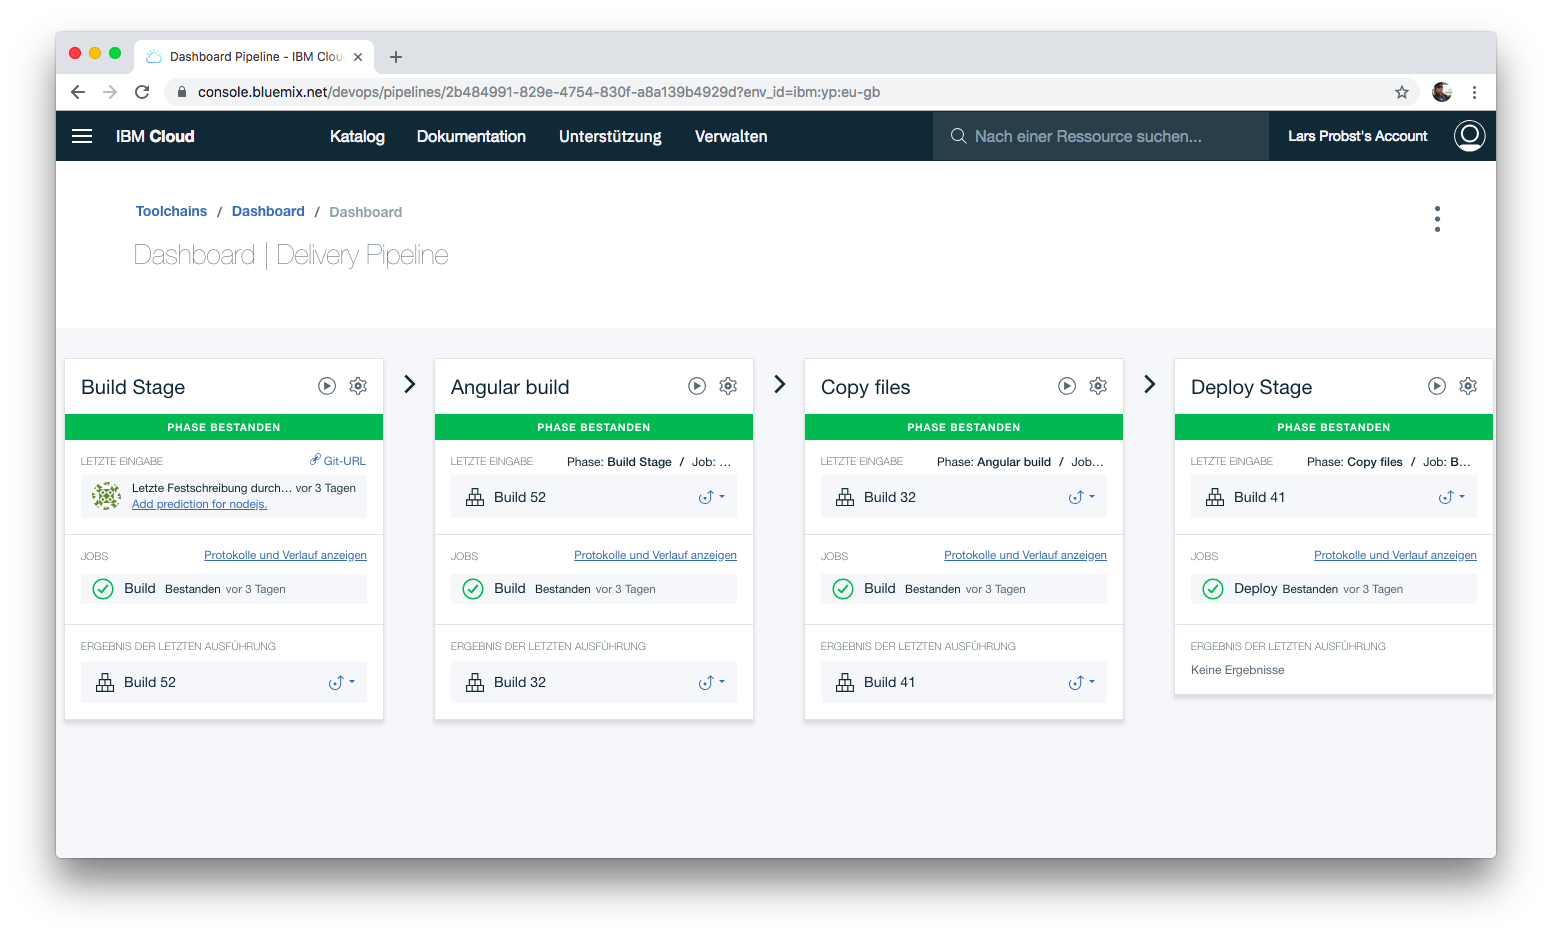
\includegraphics[width=\textwidth]{images/kapitel_3/toolchain_pipeline.png}
    \caption{Übersicht der Toolchain-Konfiguration}
    \label{fig:umsetzung_toolchain_pipeline}
\end{figure}

\subsection{API Connect}
Wie in Kapitel \ref{subsec:Aufruf mit Postman} auf Seite \pageref{subsec:Aufruf mit Postman} beschrieben, benötigt das
REST-Interface des erstellten Deployments einen Auth-Token. Dieser kann nur über den Aufruf einer anderen
REST-Schnittstelle zur Verfügung gestellt werden.

Damit man diese Schritte vereinfachen kann und das im weiteren Verlauf erstellte Frontend ebenfalls das Deployment aufrufen
kann, werden beide Abfragen in API Connect gebündelt.

Ein weiterer Grund für das Bündeln der beiden Anfragen an den Watson Service ist das mitschicken des Benutzernamens und
des zugehörigen Passwortes zum generieren des Tokens. Damit diese Daten nicht in der zu entwickelnden Anwendung hinterlegt
werden müssen, können diese Zentral in API-Connect gespeichert werden.

Das hat den Vorteil, dass man sie bei Bedarf nur an einer zentralen Stelle abändern muss. Desweiteren ist es relativ
einfach Daten auszulesen, die von der Anwendung an die Schnittstelle geschickt werden. Dies ermöglicht es Angreifern die
Daten für andere Zwecke zu nutzen.

Ein weiterer Vorteil für die Nutzung von API Connect ist die bündelung von mehreren Schnittstellen um Vorhersagen zu
beziehen. Aktuell ist es Möglich, die Vorhersage aus dem Deployment des Watson Studio Models zu beziehen oder die
Entwickelte Node.js-Applikation mit TensorFlow.js zu nutzen.

Mittels API Connect kann man die Aufrufe optimal verteilen oder eigene Routen für die jeweile Schnittstelle bauen.
Außerdem können Änderungen schnell und kompfortabel in einem Online-Editor angepasst werden.

\subsubsection{API Connect einrichten}
Der in Kapitel \ref{subsec:apiconnect} auf Seite \pageref{subsec:apiconnect} instanziierte Service wird im folgenden
konfiguriert und eingerichtet. Dazu muss man ihn aus dem IBM CLoud Dashboard heraus aufrufen. Nach dem klick auf den
Service-Namen erscheint eine Seite mit hilfreichen Informationen zum Service.

Über die Schaltfläche \texttt{Open API Connect} gelangt man auf das API Connect Dashboard. In diesem muss zuerst ein
automatisch angelegter Katalog benamt werden. In diesem Katalog werden alle Informationen zur API gespeichert.
Veröffentlichte APIs werden automatisch in diesem Katalog aufgelistet. Nach der fertigen Einrichtung des Kataloges gelangt
man über einen klick auf \texttt{Entwürfe} auf die Entwurfsübersicht.

In dieser muss man über den Menüpunkt \texttt{APIs} auswählen. In dieser Liste werden alle APIs, welche im weiteren
erstellt werden, aufgelistet. Aktuell existieren hier aber noch keine. Dies kann der Nutzer über den Button
\texttt{Hinzufügen} und dann \texttt{Neue API} ändern.

Nachdem man den Titel, einen Namen und eine beliebige Version hinterlegt hat, kann man die API mit \texttt{API erstellen}
in die Liste aufnehmen. Sie erscheint nun mit dem definierten Namen. Über einen klick auf diesen lässt sich die
Konfiguration der API öffnen.

Für die Konfiguration einer API existieren drei wichtige Untermenüs. In \texttt{Gestalten} lassen sich Name, Beschreibung,
Version, die Sicherheitsdefinitionen sowie die zur Verfügung gestellten Pfade und dafür vorgesehene Parameter definieren.

Der Menüpunkt \texttt{Quelle} zeigt die komplette Konfiguration der API in Swagger-Notation an. Hier getätigte Änderungen
werden automatisch in den anderen beiden Menüpunkte übernommen.

Im letzten Menüpunkt, \texttt{Assemblieren}, kann man die Funktionen der API definieren. Dazu zählen zum Beispiel die
einzelnen Schritte, welche bei einem Endpunkt durchlaufen werden müssen. Hier wird der Inhalt der API definiert.

Um mit der Konfiguration zu starten, muss der Nutzer zuallererst die einzelnen Pfade, welche zur Verfügung stehen sollen,
definieren. Dazu wird in den Menüpunkt \texttt{Gestalten} gewechselt und im linken Menü dann in \texttt{Pfade}.

Über das kleine Plus-Zeichen im rechten Bereich kann der Nutzer einen neuen Pfad hinzufügen. Pfade sind die Endpunkte
einer REST-Schnittstelle. Jede URL ist ein Endpunkt. Über jeden einzelnen Endpunkt können verschiedene HTTP-Requests
angesteuert werden. Die häufigsten sind \textit{GET}, \textit{POST}, \textit{PUT} und \textit{DELETE}.

Direkt nach einem klick auf das Plus-Zeichen erscheint ein neuer Pfad mit dem Namen \textit{/pfad-1}. Diesen kann man
durch einen klick aufklappen. Es erscheinen nun die Konfigurationsparameter für den Endpunkt. Als \textit{Pfad} wird nun
ein Name vergeben, über den das Watson Studio Deployment aufgerufen werden kann. Ein Beispiel hierfür ist
\textit{predict-watson}.

Da in der jetzigen Version für die Parameter keine Validierung vorgenommen wird, kann die Einstellung dieser ignoriert
werden. Allerdings muss man nun eine neue Operation hinzufügen. Dabei handelt es sich um die HTTP-Typen. Da von der
späteren Anwendung Daten an die Schnittstelle geschickt werden sollen, muss es eine Operation vom Typ \textit{POST} sein.

Über den Button \texttt{Operation hinzufügen} kann man diese hinzufügen. In dem Dropdown-Menü muss der Nutzer dann den
entsprechenden \texttt{POST}-Eintrag auswählen. Dieser erscheint sogleich in der Liste und wird grün hinterlegt.

Mit einem Klick auf den Eintrag wechselt man in die weitere Konfiguration. Die weitere Konfiguration ist für die
Schnittstelle uninteressant und kann wieder geschlossen werden.

Diese Schritte muss man nun auch für einen weiteren Pfad mit dem Namen \textit{predict-tensorflow} durchführen. Dieser
erhält ebenfalls eine Operation \textit{POST}.

Somit sind erfolgreich zwei Endpunkt mit den Namen \textit{predict-watson} und \textit{predict-tensorflow} angelegt worden.
Diese haben jeweils eine Operation vom Typ \textit{POST}.

Als weitere wichtige Einstellung muss man unter \texttt{Lebenszyklus} den Schalter bei \texttt{CORS} aktivieren und da
im ersten Schritt mit keiner Sicherheit gearbeitet wird, kann der entsprechende Menüpunkt übersprungen werden.

Über das Disketten-Symbol am oberen Rand kann man die aktuelle Einstellung zur Sicherheit speichern. Eine entsprechende
Meldung quittiert die Speicherung.

Die Grundeinstellungen der Schnittstelle sind somit getätigt. Im weiteren muss der Entwickler die API über Assemblieren
mit dem richtigen Verhalten versehen. Dazu wechselt man über den entsprechenden Menüpunkt in einen fast leeren
Arbeitsbereich.

Hier finden sich im linken Bereich alle möglichen Bausteine um die API mit Funktion zu füllen. Im mittleren Teil, dem
Arbeitsbereich, ist lediglich ein Punkt hinterlegt. Dies dient als Einstieg bei einem Aufruf der Schnittstelle. Ein
Aufruf der API landet immer in diesem Knoten und kann dann verteilt werden.

Als einer der ersten Schritte soll die Schnittstelle selbstständig einen Auth-Token vom Watson Studio abgreifen. Dazu
wird das Modul \texttt{Aufrufen} benötigt. Durch ein Drag\&Drop kann man dieses Modul in den Arbeitsbereich, direkt
hinter den schon hinterlegten Punkt setzen. Automatisch werden die beiden Module verbunden.

Durch ein doppelten Klick auf das Modul öffnet sich die entsprechende Konfiguration. Als Titel kann man \enquote{Get Token}
definieren. Als URL dient die Schnittstelle des Watson Studios, \enquote{https://eu-gb.ml.cloud.ibm.com/v3/identity/token}.

Der Benutzername und das zugehörige Passwort sind im instanziierten Watson Studio Service zu sehen. Man gelangt über das
IBM Cloud Dashbaord auf die Seite. Als \textit{HTTP-Methode} muss \texttt{GET} ausgewählt sein. In der Schnittstelle des
Watson Studios, existiert auf diesem Endpunkt lediglich diese Operation.

Als letzte Einstellung muss man als \textit{Antwortobjektvariable} die Bezeichnung \enquote{newtoken} eintragen. Die
Konfiguration des Modules ist damit abgeschlossen und es kann mit den nächsten Modulen fortgefahren werden.

Da die Schnittstelle des Watson Studios den Auth-Token als Rückgabeparameter besitzt, muss man diesen in API Connect
speichern und allgemein zur Verfügung stellen. Dies kann nur über das Modul \texttt{Zuordnen} erfolgen.

Dieses Modul kann man der Kategorie \textit{Umwandlungen} entnehmen und es direkt nach dem Request-Modul platzieren. Es
reiht sich somit dahinter ein. Ein doppelter Klick öffnet die Konfiguration des Modules. Da hier nur ein Parameter
gespeichert werden muss, ist die Konfiguration recht simpel.

In der Spalte Eingabe kann man über den Stift einen neuen Eintrag hinzufügen. Als Kontextvariable ist
\enquote{newtoken.body.token} zu definieren. Dabei handelt es sich um den Rückgabeparameter des vorangestellten
Request-Modules und das JSON-Object \enquote{token}, welches von der Schnittstelle zurückgegeben wird.

Als Name der Variable wird \enquote{Token Input} definiert, der Inhaltstyp ist \enquote{text/plain} und die Definition
ist \enquote{string}. Über \texttt{Fertig} kann man die Konfiguration speichern.

Nun muss in der Spalte Ausgabe eine interne Variable definiert werden, welche den Auth-Token speichert. Dafür wird über
den Stift ein neuer Eintrag angelegt. Die Kontextvariable ist \enquote{newtoken} und der Name \enquote{Token Output}.
Als Inhaltstyp wird \enquote{text/plain} ausgewählt, da die Variable auf der Seite der Eingabe als Text definiert ist.
Somit wird auch die Definition auf \enquote{string} gesetzt.

Nachdem auf beiden Seiten nun ein Eintrag erscheint, muss man diese beiden über die rundlichen Punkte verbinden. Eine
grüne Linie symbolisiert anschließend die Verbindung. Die Konfiguration der Zuordnung ist damit fertiggestellt.

Da bei der Schnittstelle mir CORS gearbeitet wird, muss man in einem nächsten Schritt den Header setzen, welche Anfragen
erlaubt sind. Dafür verwendet man einen \textit{Gateway Script}. Dies platziert man einfach hinter dem Zuordnungs-Modul.

Die Konfiguration des Moduls entspricht Quellcode in JavaScript. Die Zeilen in Listing \ref{Gateway Script für CORS} auf
Seite \pageref{Gateway Script für CORS} definieren die entsprechenden Einstellungen.

\begin{lstlisting}[language=JavaScript, caption=Gateway Script für CORS, label=Gateway Script für CORS]
// Set CORS headers
apim.setvariable('message.headers.Access-Control-Allow-Origin', '*');
apim.setvariable('message.headers.Access-Control-Allow-Headers', 'Origin, X-Requested-With, Content-Type, Accept');
\end{lstlisting}

Die zweite Zeile besagt, dass die nachfolgende Konfiguration für \textit{alle} Requests zählt. Die dritte Zeile besagt,
dass die Anfragen akzeptiert werden sollen. Somit kann jede Anwendung mit dieser Schnittstelle kommunizieren.

Da es zwei Endpunkte für die Schnittstelle geben wird, braucht man nun einen \textit{Operationsswitch}, um je nach
gefordertem Endpunkt auch die richtigen Informationen zurückgeben zu können.

Dieser Switch wird direkt nach dem Gateway Script angeordnet. In der Konfiguration des Switches kann der Nutzer über den
Button \texttt{+ Pfad} einen neuen Zweig hinzufügen. Insgesamt werden zwei Stück benötigt. Der erste Fall ist für
\textit{predict-watson} da. Der Zweite für \textit{predict-tensorflow}.

\subsubsection*{Pfad für das Watson Deployment}
Für den Pfad des \textit{predict-watson} wird ein weiteres Gateway Script benötigt, welches den Header für die Anfrage
an des Watson Studio Deployment setzt. Für die Einstellungen sind die JavaScript Zeilen in Listing
\ref{Gateway Script für Authorization-Token} auf Seite \pageref{Gateway Script für Authorization-Token} zuständig.

\begin{lstlisting}[language=JavaScript, caption=Gateway Script für Authorization-Token, label=Gateway Script für Authorization-Token]
// Set the token
var token = apim.getvariable('newtoken');
apim.setvariable('message.headers.authorization', 'Bearer ' + token);
\end{lstlisting}

In der zweiten Zeile wird der Token, welcher in dem Modul \textit{Zuordnung} gespeichert wurde, ausgelesen. Die dritte
Zeile sorgt dafür, dass ein Header mit dem Key \textit{authorization} und dem Value \textit{Bearer + token} gesetzt wird.

Ein weiteres Gateway Script sorgt dafür, dass die ursprünglich Übergebenen Parameter an den API Connect Service (mit den
Input-Werten für die Vorhersage) auch an den nächsten Request weitergegeben werden können. Dafür setzt man die alten Werte
als neue Message-Werte. Das Listing \ref{Gateway Script zum setzen des Message-Bodys} auf Seite
\pageref{Gateway Script zum setzen des Message-Bodys} veranschaulicht das vorgehen.

\begin{lstlisting}[language=JavaScript, caption=Gateway Script zum setzen des Message-Bodys, label=Gateway Script zum setzen des Message-Bodys]
// Get variables
var request = apim.getvariable('request.body');
apim.setvariable('message.body', request);
\end{lstlisting}

Im letzten Schritt muss man ein weiteres Aufruf-Modul hinzufügen. Dies erledigt den eigentlichen Aufruf an das Watson
Studio Deployment. Dazu wird das Modul als das Nächste in die Reihe eingefügt. In der Konfiguration muss man lediglich
die URL des Deployments hinzufügen. Diese ist auf der Seite des Deployments ersichtlich.

Damit ist dieser Pfad fertig konfiguriert und kann mit einem Aufruf verifiziert werden.

\subsubsection*{Pfad für den TensorFlow Container}
Die Einrichtung des TensorFlow-Pfades ist sehr ähnlich zum vorherigen Pfad. Allerdings bedarf es keines Gateway Scriptes
zum setzen eines Authorization Tokens, da dieser hier nicht benötigt wird. Die anderen Module kann man kopieren und in
dem Pfad einsetzen. Lediglich das Aufrufen-Modul benötigt weitere Konfiguration.

In diesem muss nicht die URL des Watson Studio Deployments, sondern man muss die des Cloud Foundry-Containers einsetzen.
Anschließend sollte man die Konfiguration über das Disketten-Symbol speichern. Die Konfiguration des API Conenct Services
ist somit abgeschlossen und man kann diese im eingerichteten Katalog veröffentlichen.

\subsubsection{API Veröffentlichen}
In der Abbildung \ref{fig:umsetzung_api_connect} auf Seite \pageref{fig:umsetzung_api_connect} ist der fertig eingerichtete
API Connect flow dargestellt.

\begin{figure}[h]
    \centering
    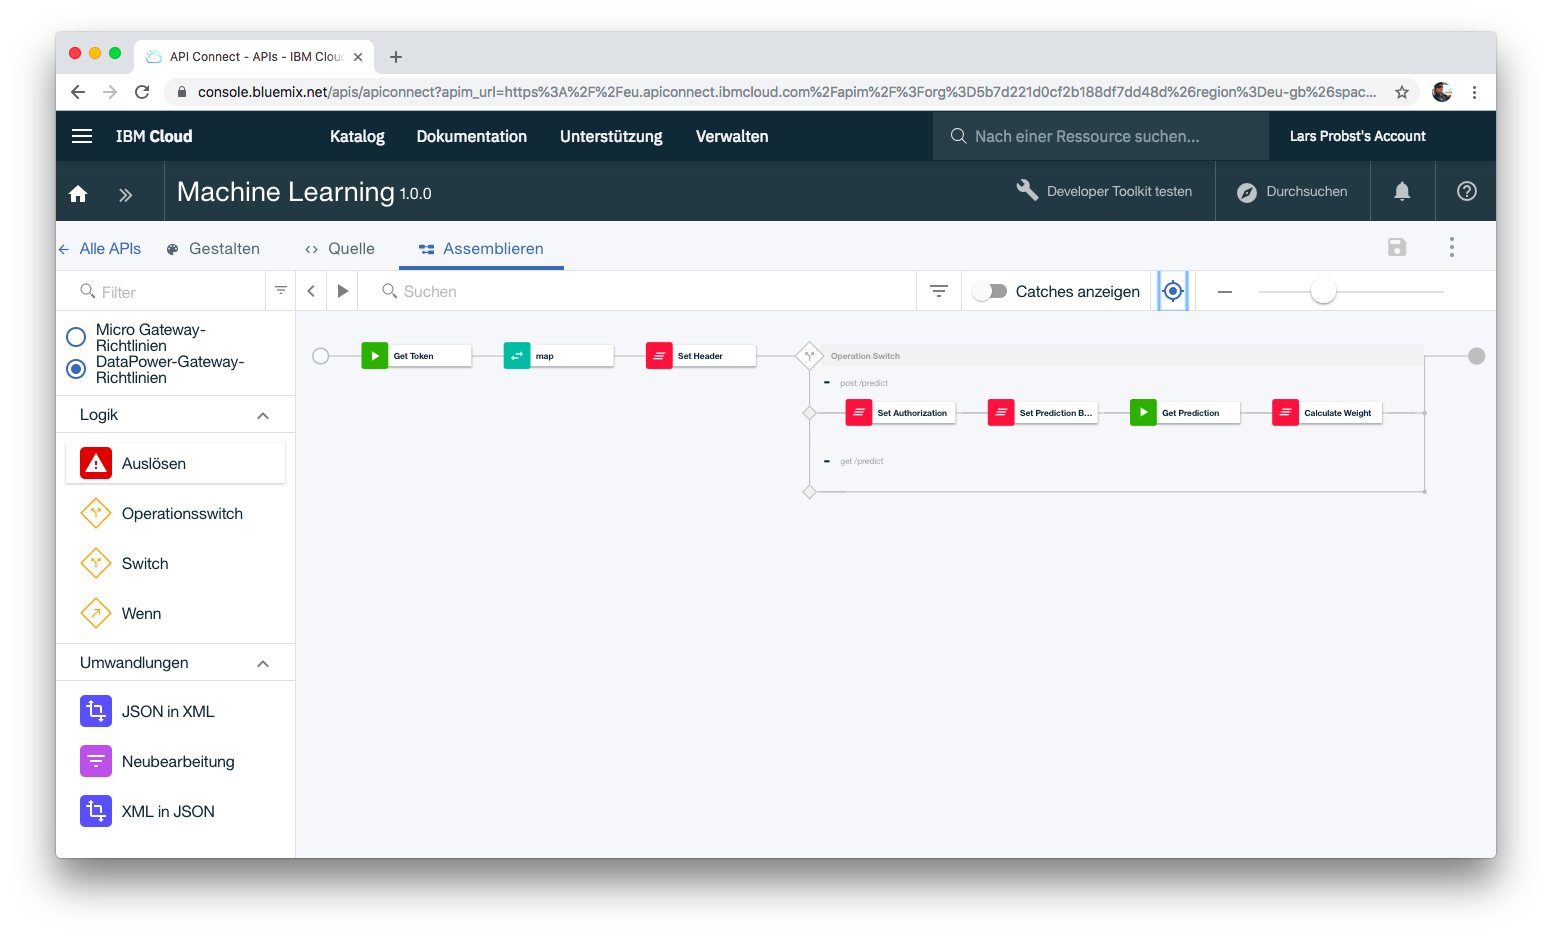
\includegraphics[width=\textwidth]{images/kapitel_3/api_connect.png}
    \caption{Kompletter API Connect flow}
    \label{fig:umsetzung_api_connect}
\end{figure}

Über den Play-Button am linken oberen Rand, kann man die aktuelle Konfiguration des API Connect Services bauen lassen.
Als Katalog sollte man den anfangs angelegten Katalog definieren. Im Bereich Produkt muss der Nutzer ein neues anlegen.

Nun kann er mit \texttt{Produkt veröffentlichen} dieses veröffentlichen und nutzbar machen. Dieser Vorgang kann bis zu
wenigen Minuten dauern.

\subsubsection{API Durchsuchen}
Man kann auf Durchsuchen klicken und dann sieht man die Swgaer UI und kann die API auch testen etc...
\colorbox{yellow}{Hier fehlt was}

\subsubsection{Developer Toolkit}
Hier kann man Informationen zur API sehen und sowas...
\colorbox{yellow}{Hier fehlt was}